\documentclass[cic,tc,english]{iiufrgs}
% Para usar o modelo, deve-se informar o programa e o tipo de documento.
% Programas :
% * cic       -- Graduação em Ciência da Computação
% * ecp       -- Graduação em Ciência da Computação
% * ppgc      -- Programa de Pós Graduação em Computação
% * pgmigro   -- Programa de Pós Graduação em Microeletrônica
% 
% Tipos de Documento:
% * tc                -- Trabalhos de Conclusão (apenas cic e ecp)
% * diss ou mestrado  -- Dissertações de Mestrado (ppgc e pgmicro)
% * tese ou doutorado -- Teses de Doutorado (ppgc e pgmicro)
% * ti                -- Trabalho Individual (ppgc e pgmicro)
% 
% Outras Opções:
% * english    -- para textos em inglês
% * openright  -- Força início de capítulos em páginas ímpares (padrão da
% biblioteca)
% * oneside    -- Desliga frente-e-verso
% * nominatalocal -- Lê os dados da nominata do arquivo nominatalocal.def

\newcommand{\bruno}[1]{\textcolor{red}{\textbf{#1}}}
\newcommand{\adriano}[1]{\textcolor{blue}{\textbf{#1}}}
\newcommand{\pergunta}[1]{\textcolor{green}{\textbf{#1}}}

% Use unicode
\usepackage[utf8]{inputenc}   % pacote para acentuação
\usepackage[]{algorithm2e}
\usepackage{amsfonts}
\usepackage{amsmath}
% Necessário para incluir figuras
\usepackage{graphicx}         % pacote para importar figuras

\usepackage{times}            % pacote para usar fonte Adobe Times
% \usepackage{palatino}
% \usepackage{mathptmx}       % p/ usar fonte Adobe Times nas fórmulas

\usepackage[alf,abnt-emphasize=bf]{abntex2cite}    % pacote para usar citações abnt
% 
% Informações gerais
% 
\title{A Comparison of Recommender Systems for Crowdfunding Projects}

\author{Carniel Benin}{Adriano}
% alguns documentos podem ter varios autores:
% \author{Flaumann}{Frida Gutenberg}
% \author{Flaumann}{Klaus Gutenberg}

% orientador e co-orientador são opcionais (não diga isso pra eles :))
\advisor[Prof.~Dr.]{Castro da Silva}{Bruno}

% a data deve ser a da defesa; se nao especificada, são gerados
% mes e ano correntes
% \date{maio}{2001}

% o local de realização do trabalho pode ser especificado (ex. para TCs)
% com o comando \location:
\location{Porto Alegre}{RS}

% itens individuais da nominata podem ser redefinidos com os comandos
% abaixo:
% \renewcommand{\nominataReit}{Prof\textsuperscript{a}.~Wrana Maria Panizzi}
% \renewcommand{\nominataReitname}{Reitora}
% \renewcommand{\nominataPRE}{Prof.~Jos{\'e} Carlos Ferraz Hennemann}
% \renewcommand{\nominataPREname}{Pr{\'o}-Reitor de Ensino}
\renewcommand{\nominataPRAPG}{Prof.~Vladimir Pinheiro do Nascimento}
% \renewcommand{\nominataPRAPGname}{Pr{\'o}-Reitora Adjunta de P{\'o}s-Gradua{\c{c}}{\~a}o}
% \renewcommand{\nominataDir}{Prof.~Philippe Olivier Alexandre Navaux}
% \renewcommand{\nominataDirname}{Diretor do Instituto de Inform{\'a}tica}
\renewcommand{\nominataCoord}{Prof.~Sérgio Luis Cechin}
% \renewcommand{\nominataCoordname}{Coordenador do PPGC}
% \renewcommand{\nominataBibchefe}{Beatriz Regina Bastos Haro}
% \renewcommand{\nominataBibchefename}{Bibliotec{\'a}ria-chefe do Instituto de Inform{\'a}tica}
% \renewcommand{\nominataChefeINA}{Prof.~Jos{\'e} Valdeni de Lima}
% \renewcommand{\nominataChefeINAname}{Chefe do \deptINA}
% \renewcommand{\nominataChefeINT}{Prof.~Leila Ribeiro}
% \renewcommand{\nominataChefeINTname}{Chefe do \deptINT}

% 
% palavras-chave
% iniciar todas com letras minúsculas, exceto no caso de abreviaturas
%
\keyword{machine learning}
\keyword{recommender systems}
\keyword{AI}
\keyword{crowdfunding}

%\settowidth{\seclen}{1.10~}

% 
% inicio do documento
% 
\begin{document}

% folha de rosto
% às vezes é necessário redefinir algum comando logo antes de produzir
% a folha de rosto:
% \renewcommand{\coordname}{Coordenadora do Curso}
\maketitle

% dedicatoria
\clearpage
\begin{flushright}
    \mbox{}\vfill
    {\sffamily\itshape
      ``The question of whether computers can think\\
      is like the question of whether submarines can swim.''\\}
    --- \textsc{Edsger W. Dijkstra}
\end{flushright}

% agradecimentos
\chapter*{Acknowledgments}
%Agradeço ao \LaTeX\ por não ter vírus de macro\ldots
\begin{abstract}
    Recommender systems have been a popular research topic in the field of Machine Learning and are of great commercial interest for many businesses. This work aims to implement and evaluate different recommendation strategies in the context of a crowdfunding platform. The main approaches used in modern commercial applications will be considered in this work and several performance metrics will be measured in order to evaluate each implemented recommendation system. The crowdfunding platform in which we evaluate these different recommendation algorithms provides many interesting challenges, such as the transient nature of projects and the low amount of information available for rating prediction. Results from production tests with real users will be provided in order to compare each approach with a chosen baseline.
\end{abstract}
%%TODO mudar para portugues
%\begin{otherlanguage}{english} 
\begin{englishabstract}{Uma Comparação de Sistemas de Recomendação para Projetos de Financiamento Coletivo}{aprendizado de máquina. sistemas de recomendação. IA. financiamento coletivo}

Sistemas de recomendação são um tópico de grande interesse de pesquisa na área de aprendizado de máquina e são de grande interesse comercial para vários negócios. Esse trabalho propõe implementar e analisar diferentes estratégias de recomendação para uma plataforma de financiamento coletivo em particular. As principais abordagens empregadas em sistemas comerciais modernos serão analisadas, e várias métricas de performance serão avaliadas para cada uma delas. A plataforma de financiamento coletivo na qual avaliamos as técnicas de recomendação selecionadas apresenta diversas características que dificultam a implementação de sistemas de recomendação, tais como a natureza transiente dos projetos e a pequena quantidade de dados disponíveis para prever as avaliações dos usuários. No final, serão apresentados resultados comparando cada tipo de sistema de recomendação implementado em um sistema de produção com usuários reais. 
\end{englishabstract}
%\end{otherlanguage}


%% \centering
%% \parbox{\longest}{%
%%   \raggedright{\itshape%
%%     The question of whether computers can think \\
%%     is like the question of whether submarines can swim.\par\bigskip
%%   }   
%%   \raggedleft\Large\MakeUppercase{Edsger W. Dijkstra}\par%
%% }

%% \vfill\vfill

% resumo na língua do documento
%% \begin{abstract}
%%     Este documento é um exemplo de como formatar documentos para o
%%     Instituto de Informática da UFRGS usando as classes \LaTeX\
%%     disponibilizadas pelo UTUG\@. Ao mesmo tempo, pode servir de consulta
%%     para comandos mais genéricos. \emph{O texto do resumo não deve
%%       conter mais do que 500 palavras.}
%% \end{abstract}

% resumo na outra língua
% como parametros devem ser passados o titulo e as palavras-chave
% na outra língua, separadas por vírgulas
%% \begin{englishabstract}{Using \LaTeX\ to Prepare Documents at II/UFRGS}{Electronic document preparation. \LaTeX. ABNT. UFRGS}
%%     This document is an example on how to prepare documents at II/UFRGS
%%     using the \LaTeX\ classes provided by the UTUG\@. At the same time, it
%%     may serve as a guide for general-purpose commands. \emph{The text in
%%       the abstract should not contain more than 500~words.}
%% \end{englishabstract}

% lista de figuras
\listoffigures

% lista de tabelas
\listoftables

% lista de abreviaturas e siglas
% o parametro deve ser a abreviatura mais longa
\begin{listofabbrv}{MAE}
    \item[RS] Recommender System
    \item[CB] Content-based
    \item[CF] Collaborative filtering
    \item[MSE] Mean-squared error
    \item[MAE] Mean absolute error
\end{listofabbrv}

% idem para a lista de símbolos
% \begin{listofsymbols}{$\alpha\beta\pi\omega$}
%     \item[$\sum{\frac{a}{b}}$] Somatório do produtório
%     \item[$\alpha\beta\pi\omega$] Fator de inconstância do resultado
% \end{listofsymbols}

% sumario
\tableofcontents

%% \section{Figuras e tabelas}

%% Esta seção faz referência às Figuras~\ref{fig:estrutura},~\ref{fig:ex1} e~\ref{fig:ex2}, a título de exemplo. A primeira figura apresenta a estrutura de uma figura. A \emph{descrição} deve aparecer \textbf{acima} da figura. Abaixo da figura, deve ser indicado a origem da imagem, mesmo se essa for apenas os autores do texto.

%% A Figura~\ref{fig:ex1} representa o caso mais comum, onde a figura propriamente dita é importada de um arquivo ( neste exemplo o formato é \texttt{eps} ou \texttt{pdf}. Veja a seção \ref{sec:fig_format}). A Figura~\ref{fig:ex2} exemplifica o uso do environment \texttt{picture}, para desenhar usando o próprio~\LaTeX.

%% Tabelas são construídas com praticamente os mesmos comandos. Ver a tabela \ref{tbl:ex1}.


%% \subsection{Formato de Figuras}
%% \label{sec:fig_format}

%% O LaTeX permite utilizar vários formatos de figuras, entre eles \emph{eps}, \emph{pdf}, \emph{jpeg} e \emph{png}. Programas de diagramação como Inkscape (e mesmo LibreOffice) permitem gerar arquivos de imagens vetoriais que podem ser utilizados pelo LaTeX sem dificuldade. Pacotes externos permitem utilizar SVG e outros formatos.

%% Dia e xfig são programas utilizados por dinossauros para gerar figuras vetoriais. Se possível, evite-os.

%% \subsection{Classificação dos etc.}

%% O formato do instituo de informática define 5 níveis: capítulo, seção, subseção e outros 2 sem nome.

%% \subsubsection{Subsubseção}
%% Exemplo de uma subsubseção.

%% \paragraph{Parágrafo}
%% Exemplo de um parágrafo.

%% Recomenda-se o uso de bibtex para gerenciar as referências (veja o arquivo
%% biblio.bib).

% aqui comeca o texto propriamente dito

\chapter{Introduction} \label{introduction}
Since time immemorial, people have relied on recommendations from many sources to base their decisions on, be it spoken word, magazines, travel guides and so forth. The decision to buy a new book, for example, is often based on the opinions of a close group of friends; employers count on recommendation letters for recruiting; and when selecting a movie to watch, people rely on movie critics they have read. Recommender systems aim to augment this social process in order to assist people in sifting through an ever-growing list of movies, books and all sorts of items. Recommender Systems (RSs) are widely used in the industry today to provide useful suggestions to end-users in a completely automated manner. They are ubiquitous in modern e-commerce Web sites \cite{Schafer2001}, where new products can be recommended based on a customer's interests and preferences, and in many other fields such as movies (Netflix) and music (Spotify). Its importance cannot be overstated: the effectiveness of targeted recommendations, as measured by click-through and conversion rates (i.e., the ratio of users who clicked on a specific link and the total number of users who viewed a page, and the ratio of users who performed the desired final action---such as buying the product---and the number of users who viewed the page, respectively), far exceed those of untargeted content \cite{Linden2003}. By customizing recommendations for each user, search effort is greatly reduced, leading to greater customer loyalty, higher sales and advertising revenues, and better targeted promotions \cite{Ansari2000}.

A recommender system typically focuses on a specific type of "item"---the general term used to denote what the system recommends to users. The sort of items recommended by such systems can vary tremendously. Apart from the most well-known examples such as Amazon, which recommends products, and Netflix with movies, RSs are also used to recommend social connections in platforms such as Facebook, as well as news in news aggregators like Google News. Table ~\ref{tbl:system_examples} shows a list of recommender systems used in real-world applications. Some of these systems will be discussed in further details in chapter \ref{related-work}.

\begin{table}[ht!]
    \caption{Example of recommended products by various real-world applications}
    \centering
        \begin{tabular}{c|p{5cm}}
          \hline
          \textit{System}  &   \textit{Product}  \\
          \hline
          \hline
Amazon.com   & Books and other products  \\
Netflix  & DVDs, Streaming Video  \\
Jester  & Jokes  \\
GroupLens  & News  \\
MovieLens  & Movies  \\
last.fm  & Music  \\
Google News  & News  \\
Google Search  & Advertisements  \\
Facebook  & Friends, Advertisements  \\
Pandora  & Music  \\
YouTube  & Online videos  \\
Tripadvisor  & Travel products  \\
IMDb  & Movies  \\
          \hline
        \end{tabular}
    \legend{Source: \cite{Aggarwal2016}}
    \label{tbl:system_examples}
\end{table}


The mathematical objective of the recommendation problem can be formulated in a number of ways. Aggarwal et al. \cite{Aggarwal2016} propose the following main models/objectives:
\begin{itemize}
\item \emph{Prediction}: In this approach, we try to predict the rating value for a user-item combination; in particular, given a list $J$ of items and a history of past ratings given by user $i$ to various items $J_i \subset J$, we estimate the ratings that this user would give to any other items $j \not\in J_i$. The training data, based on which the RS will be trained, is given by an incomplete $R_{MxN}$ matrix, where $M$ is the number of users and $N$ the number of items. In this matrix, each entry $(i,j)$ represents the rating given by user $i$ to item $j$. This matrix is extremely sparse in most cases since most users only rate a very small subset of the available items. The observed values, which indicate user preferences for items, are used to train a model which will try to fill in the missing or unobserved ratings in the matrix. Since we have an incompletely specified matrix of values, this problem is sometimes referred to as the \textit{matrix completion problem}.
\item \emph{Ranking}: For many applications, it is not necessary to obtain absolute numerical values for the predicted ratings. Instead, we are more interested in obtaining the top-k items to recommend to a user, or the top-k users to promote a particular item. Both methods are exactly analogous, with the former being much more common in practice. This problem is often referred to as the \textit{top-k recommendation problem}.
\end{itemize}

The first formulation of the problem is more general since it is possible to derive the second one by predicting ratings for every item and then ranking the predictions. However, in many cases, it is easier and more practical to solve the ranking problem directly.

Along with the definition or objective of the problem, it is important to define the desired operational and technical characteristics of recommender systems. The main desired properties of any recommendation algorithm are as follows:
\begin{itemize}
\item \emph{Relevance}: The main goal in recommender systems is to provide recommendations that are relevant to the user at hand. Users are much more likely to consume items which they find interesting and are tailored for them.
\item \emph{Novelty}: Users are much more engaged when confronting items they have not seen in the past. Recommending the same items over and over, however good the recommendations may be, is not a good strategy.
\item \emph{Serendipity}: Serendipity in recommender systems happens when recommendations are somewhat surprising or unexpected to the user, as opposed to obvious recommendations. It differs from the concept of Novelty in that it does not simply recommend items the user did not know about before but allows the user to discover entirely new areas of interest. For example, recommending a new spicy Mexican restaurant to someone who regularly visits Mexican restaurants may be novel, but it is not surprising at all. Recommending a Thai restaurant instead might allow the user to discover a whole new interest, increasing sales diversity and user satisfaction.
\item \emph{Diversity}: Recommender systems usually suggest a list of top-k items to the user. If all the recommended items are similar, there is an increased chance that the user will not like any of the items. On the other hand, if we show diversified items there is a higher chance that the user will like at least one of them.
\end{itemize}

Additionally, we can define the main \emph{goals} of the system as a whole from the perspective of the service provider. There are many reasons why service providers may wish to invest in RSs \cite{N.N2010} \bruno{essa citacao ta estranha. Qual o nome do autor? so aparece as iniciais}:
\begin{itemize}
\item \emph{Increase sales}: Arguably the most important goal for a commercial RS, this can be achieved because recommended items are more likely to suit the user's needs than a generic non-personalized item list. In general, the primary goal of a RS is to increase the conversion rate, i.e., the number of items consumed in relation to the number of page views.
\item \emph{Diversify sales}: In a movie rental system such as Netflix, for instance, the service provider is interested in renting all of its catalog instead of just the most popular movies. However, advertising relatively unknown movies to all its user base could be risky. A RS can alleviate this problem by providing different recommendations for each user, thus increasing the effectiveness of the advertisement. 
\item \emph{Increase user satisfaction}: By providing interesting and relevant recommendations, RSs can improve the experience of the user with the application, therefore increasing the user's evaluation of the system.
\item \emph{Increase user fidelity}: The more a user interacts with a RS the more refined its user model becomes, giving them the feeling of being recognized as a valuable visitor.
\item \emph{Understand user needs}: The output of a RS can be used for many other purposes such as improving the management of an item's stock or creating promotions targeting specific user segments.
\end{itemize}

\section{Motivation} \label{motivation}
The objective of this work is to develop, evaluate and compare different state-of-the-art approaches for building RSs in the context of a particular crowdfunding platform---Catarse---of which the author is a developer.

Launched in January 2011, Catarse was the first crowdfunding platform for creative projects in Brazil. With over 7000 successfully financed projects raising R\$77m from 480.000 people, it is currently the largest national platform of its kind. It works similarly to most crowdfunding platforms: the project owner presents his or her idea for a project which they wish to be funded and specifies the required investment as well as the cutoff date for the project while offering rewards for those who back it. Projects are divided into 3 main categories: all-or-nothing, flexible, and recurrent. In the first type, projects are available for backing (i.e., to start receiving pledges from supporters) up to 60 days, and the project owner only receives the raised amount if the project's goal (total required amount of money for developing it) is met; otherwise all the money is returned to its original backers. On flexible projects, the owner receives the raised amount whether the goal was reached or not. Recurrent projects are subscription-based and the owner can collect the money monthly. 

Catarse's business model relies on charging a fixed percentage of the total pledged amount from successful projects, even if this amount is greater than the original goal. Failed projects, i.e. projects that did not meet their goal by the deadline, represent a major financial cost to Catarse since transaction fees involved in the refund process are fully absorbed by the company. Therefore, we expect to benefit from RSs in two ways: first, by increasing the average pledged amount per project, which can be achieved by presenting appropriate projects that are tailored for the user; and secondly, by increasing project discoverability we expect that more projects will be successfully funded and fewer projects will fail. \bruno{nesse trabalho tu so avalia se o 1o caso acontece, ne? de repente clarifica isso aqui com uma frase tipo 'In this work we focus on evaluating different RS strategies for improving the first above-mentioned goal'} \adriano{na secão de métricas online avalio os dois casos}

As of April 2018, over 1500 projects in 18 different categories are online and available for backing in Catarse. It would be unreasonable to expect users to browse through all projects before deciding which ones to back. For this reason, some sort of ranking is fundamental when showing projects to users, and there is no doubt that the choice of this ranking method will greatly affect conversion rates and successful funding of projects. At the time of this writing, several ranking strategies are in use. First, on the home page projects are shown ordered by popularity, defined here simply by the pledged(contributed) amount in the last 48 hours. Another section of the website shows which projects were backed by particular Facebook friends of the user, for those users who opted to connect their Facebook account to their Catarse account. Finally, on the \emph{explore page}, we also have filters for displaying projects expiring soon. It should be noted that none of these sections of the Catarse website, with the exception of the backed by friends section, display projects that are tailored for each specific user: every user will see the same projects in the same order.

Given the above properties and goals of Catarse, project recommendation can be considered a crucial aspect of Catarse's business model. We can expect any marginal improvement in this regard to be of great benefit to the company and its users. Therefore, a user-tailored recommendation system is fundamental to stay competitive in this market and is expected to greatly increase user satisfaction, both for backers who will be able to more easily find projects that are interesting to them, and for project owners who will receive more visits to their projects due to increased discoverability.

Catarse's dataset is unique in a variety of ways that makes collaborative filtering (CF) techniques (explained later in Chapter \ref{background}) hard to apply. First, unlike regular e-commerce Web sites such as Amazon, where products stay available for many years, crowdfunding projects have a predetermined cutoff date, after which it is no longer possible to make a pledge. It makes no sense to recommend expired projects, limiting our possible recommendations to online \bruno{active?} \adriano{online é o termo mais usual em crowdfunding, adicionei na secão de terminologia} projects only. Another challenge is the fact that the majority of Catarse's users only back one project, thus making it hard to collect enough data for CF methods to work properly. One typical characteristic of classic CF systems is that they may have to be retrained after every new interaction; this imposes scalability challenges when implemented on highly dynamic data, such as the training data of Catarse. On the other hand, content-based methods (discussed in Chapter \ref{background}) allows us to train our model with the whole dataset in order to extract backer-project features only once, and later use this model to search for online projects with the highest backing probability for the current user. However, such methods also have drawbacks, as discussed in Chapter \ref{background}. These challenges motivate us to search for methods that are adequate to our specific needs.

\section{Goals}
This work aims to implement and compare the main computational strategies for building RSs and apply them in the context of a particular large-scale Crowdfunding website. Several metrics will be used to determine the best approach, which will then be deployed in a production environment. Our primary goal is to find a strategy that is at least better than the current-used popularity ranking, which is usually hard to beat in realistic scenarios.

\section{Definitions and Terminology}

We present, below, some crowdfunding-specific definitions and terminology that will be used throughout this work:
\begin{itemize}
\item \textbf{Contribution, pledge or back}: financial endorsement by a user to a specific project;
\item \textbf{Backer}: a platform user that contributed to a project;
\item \textbf{Project Owner}: the user that created the project;
\item \textbf{Successful Project}: a project that, by the end of its deadline, has reached its goal;
\item \textbf{Failed Project}: a project that, by the end of its deadline, has not reached its goal;
\item \textbf{Online Project}: a project that is available for backing and has not yet reached its deadline;
\item \textbf{Reward}: something that is offered or promised to backers for contributing to the project;
\end{itemize}

\section{Structure}

This work is divided into 6 chapters. In the first chapter, the basic concepts of Recommender Systems are discussed, as well as the motivation and goals underlying this work. In the second chapter, we analyze a few existing applications that rely on Recommender Systems. On the third chapter, theoretical background for the employed methods is presented. The fourth chapter describes how we conducted our experiments. In the fifth chapter experimental results are presented and discussed. Finally, in the sixth chapter we summarize our conclusions and describe future work.

\chapter{Related Work} \label{related-work}

In this chapter, a few selected existing commercial applications of RSs will be discussed. For each application, the relevant underlying RS techniques (some of which will later be used in our own implementation) are highlighted and a brief explanation of how they were applied to that system (or how they differ from our use-case platform) is provided. Details on how each technique can be computationally implemented are discussed later on in Chapter \ref{background}.

\section{GroupLens Recommender System}
One of the first recommender systems to be developed, Grouplens \cite{N.N2010} was used for recommendations of Usenet news. It worked by collecting ratings from many Usenet readers in order to recommend new articles to users, a technique now known as Collaborative Filtering (CF). This technique will be discussed in more details in Section \ref{cf}.

This basic approach was later extended to other settings such as ones for recommending books and movies; these were referred to as Booklens and Movielens, respectively. One important contribution of this research was the release of several datasets of user ratings to the research community, which were not easily available at the time. One of these datasets, Movielens, is still widely used in RS research to this day.

Collaborative filtering techniques such as the ones used by GroupLens remain one of the most popular approaches for building RSs to this day. In our implementation, this technique will be used to recommend projects to users by collecting implicit ratings from users; \bruno{in the context of our crowdfunding project, the act of backing a project counts as a positive rating to that project}. \bruno{nao sei se isso ta re-explicado depois, em outras secoes, quando tu fala de positive ratings no contexto do catarse, mas talvez fosse bom mencionar novamente nas secoes seguintes relevantes, porque senao essa explicacao importante sobre o teu sistema vai ficar perdida no final de um paragrafo descrevendo o trabalho de outra pessoa}

\section{Netflix Recommender System}
Netflix recommendations are obtained through user ratings on a 5-point scale (recently changed to a thumbs up/down system) as well as implicit ratings, such as the action of watching a movie. One interesting aspect of their system is the quality of explanations provided to the recommendations. For instance, a list of recommendations can be pinpointed to having watched a specific movie. This approach can help users decide what to watch and also contribute to improving customer loyalty and retention.

The Netflix Prize contest was a competition organized by Netflix that ran from 2006 to 2009. Contestants were given a data set of (real-life anonymized) existing user ratings for different movies and were expected to outperform Netflix's own recommendation algorithm, Cinematch. This contest was responsible for many notable contributions to recommendation systems' research, such as advancements in latent factor models. Many of these contributions were applied in the algorithms used in this work.

\section{Kickstarter Recommender System}
Kickstarter is the world's largest crowdfunding platform and works very similarly to Catarse, making it a great reference for our implementation. Kickstarter's initial implementation of its recommender system used a Collaborative Filtering approach, written entirely in MySQL. Later, Content-Based recommendations (discussed in Section \ref{cb}), which are based on the similarity of the text, were used by Kickstarter and implemented via a method called Latent Semantic Indexing (LSI). Both these approaches were later combined into the current Hybrid system. For the initial tests performed by Kickstarter, the "popular projects" ranking was used as a baseline for comparing new algorithms. \adriano{This ranking order projects by their total pledged amount in the last 24 hours.}

Due to the similarity between Kickstarter and Catarse's platform we can expect that a similar RS implementation could work equally well. In fact, in our work we evaluate many of the techniques used by Kickstarter, such as CF-based RSs, CB-based RSs, and a hybrid approach. Similarly to Kickstart, our performance evaluation will also be (partially) based on comparisons to the existing popularity metric. However, some key differences between the platforms must be taken into account when designing a RS for Catarse. Specifically, flexible projects, which do not exist on Kickstarter, must be taken into consideration due to their distinct funding and time characteristics and constraints. These considerations are further discussed in Chapter \ref{experiment}.

\chapter{Theoretical Background} \label{background}
In this chapter, the main concepts behind Recommender Systems will be reviewed. We will discuss the most common approaches used in the industry today and provide a detailed comparison of their general characteristics, as well as insights that are relevant to our particular application. For each general approach for constructing a RS, we give descriptions of the most used algorithms along with state-of-the-art techniques that were selected for use in the experiments that we conduct (see Section \ref{experiment}).

The basic idea behind any recommender system is to obtain a utility function to estimate user preferences towards an item. The meaning of this function will differ for each context; it could mean how likely a user will want to watch a specific movie or listen to a song, or the likelihood of buying a particular product. In our case, the goal is to find projects the customer is most likely to back given his backing history and other characteristics. 

Methods for implementing Recommender Systems can be broadly divided into two categories: \textbf{Content-Based} (CB) and \textbf{Collaborative Filtering} (CF) methods \cite{Rakesh2016}.
The former utilizes user features and content features (describing items, such as relevant keywords) in order to recommend items to users. In collaborative filtering methods, user ratings are used in order to calculate similarities between users (user-based CF) or between items (item-based CF), which are then ranked in order to show the most relevant recommendations to each specific user by exploiting inter-user and inter-item relationships. How these similarities are computed and used to rank items is described in section \ref{cf}. Content-Based models also utilize user ratings in most cases; however, the model usually focuses on predicting the ratings of a single user, instead of attempting to discover inter-user relationships. These two methods are sometimes combined into what is known as Hybrid Recommender Systems. Hybrid systems can combine the strengths of various models in order to perform more robustly in a wide variety of settings.

In the next sections, mathematical models for these approaches will be provided, as well as a discussion of their main advantages and shortcomings.

\section{Collaborative Filtering} \label{cf}
Collaborative filtering (CF) is based on the principle that similar users will share similar interests. Assuming that ratings are highly correlated across various users and items, it is possible to predict a rating not yet given by the user. For example, if the algorithm identifies that user Alice and Bob have similar tastes, even if only Alice rated a certain item, we can surmise that Bob would give a similar rating as hers. 

CF algorithms can be divided into two categories: \textbf{Memory-Based} and \textbf{Model-Based} approaches. Memory-Based CF algorithms, also referred to as \textit{neighborhood-based collaborative filtering algorithms}, represent each customer by a \(N\)-dimensional vector of item ratings, where \(N\) stands for the number of available items, and where each vector component corresponds to the user rating of the corresponding item. These ratings can be obtained explicitly --- e.g. star rating or "likes" --- or implicitly --- e.g. a user buying an item or listening to a song can be considered a positive rating. By collecting ratings from $M$ users, we build a \(R_{n \times m}\) matrix which is the starting point for Memory-Based CF. Each entry $R_{ij}$ in this matrix corresponds to an observed rating by user $i$ to item $j$, while missing ratings are represented with some sort of null value. For most applications, $R$ will be extremely sparse. Our job is to try to predict the missing ratings; for this to be possible, most models focus on leveraging inter-item or inter-user correlations, that is, the similarities between items or between users. Memory-Based methods were among the earliest CF methods proposed. Although very simple to implement, these methods often have trouble with very sparse matrices, since they use the $R$ matrix directly to compute similarities and make predictions, which is often very large. Neighborhood methods are discussed in section \ref{neighbourhood}.

In Model-Based CF methods, on the other hand, machine learning and data mining algorithms are used to develop a model based on the $R$ ratings matrix that will be used to predict user ratings. Some examples include decision trees, rule-based models, Bayesian methods and latent factor models. These methods can solve some of the shortcomings of Memory-Based approaches, such as the need for large rating matrices since they use a pre-computed model instead of directly using the $R$ matrix to make predictions, often by means of dimensionality reduction of the $R$ matrix. Finally, both approaches can be combined into Hybrid Recommenders. An overview of these techniques is depicted in figure ~\ref{fig:cf-comparison}.

\subsection{Neighborhood Methods for CF} 
\label{neighbourhood}
    Neighborhood methods take rows or columns of $R$ and compute a similarity value between them. If the rows correspond to users and the columns to items, we can obtain the similarity between two users $u$ and $v$ by computing the correlation between the rows $u$ and $v$ of $R$. This is usually referred to as \textit{User-Based CF}. In the same fashion, the similarity between items $i$ and $j$ can be computed by taking columns $i$ and $j$ of $R$ and calculating their distances, which is referred to as \textit{Item-Based CF}.

For User-Based CF, given rows corresponding to users $u$ and $v$ in the $R$ matrix, one common method to compute similarity between users is the cosine measure given by:

$$sim( u,  v) = \cos( u,  v) = \frac { u \cdot  v}{|| u|| \cdot || v||} = \frac{\sum_{i \in I_{uv}} r_{ui}r_{vi}}{\sqrt{\sum_{i \in I_u} r_{ui}^2}\sqrt{\sum_{i \in I_v} r_{vi}^2}}$$

\noindent where $I_u$ and $I_v$ are the sets of items rated by user $u$ and $v$ respectively, $I_{uv} = I_u \cap I_v$ and $r_{xi}$ is the observed rating of user $x$ to item $i$. To get a rating prediction $\check{r}_{ui}$ given by the user $u$ to item $i$, we aggregate ratings from the subset of users most similar to $u$, $U'$. One such aggregation function could be:

$$
\check{r}_{ui} = n \sum_{u' \in U'} sim(u, u')r_{u'i}
$$

\noindent where $n$ is a normalizing factor. For large databases, User-based CF can be prohibitively computationally expensive. Its worst-case performance is $O(MN)$ where $M$ is the number of customers and $N$ is the number of items \cite{Linden2003}; this problem can, sometimes, be partially alleviated by exploiting sparsity in the customer vector.

Item-Based CF works almost exactly the same as User-Based CF. One important distinction is that item-based CF retrieves recommendations directly from the similarity matrix and does not require $R$ to be kept in memory. A major reason for the adoption of this approach is that in most systems users are much more numerous than items, leading to a significantly reduced similarity matrix when using item-based CF \cite{Sarwar2001}. We can redefine the cosine measure for this case like so: let $U_i$ and $U_j$ be the set of users who rated items $i$ and $j$ respectively, and $U_{ij} = U_i \cap U_j$ be the set of users who rated both items $i$ and $j$, the similarity is then given by:


$$sim( i,  j) = \cos( i,  j) = \frac { i \cdot  j}{|| i|| \cdot || j||} = \frac{\sum_{u \in U_{ij}} r_{ui}r_{uj}}{\sqrt{\sum_{u \in U_i} r_{ui}^2}\sqrt{\sum_{u \in U_j} r_{uj}^2}}$$

Similarly, we define the rating prediction for item-based CF, considering $J$ to be the set of items $j$ most similar to $i$, as:

$$
\check{r}_{ui} = \frac{\sum_{j \in J} sim(i, j)r_{uj}}{\sum_{j \in J} sim(i, j)}
$$

Item-based CF was first proposed by Amazon \cite{Linden2003}. Each item purchased by the customer is compared to other items in the dataset in order to calculate a similarity metric. The original algorithm is shown below:

\begin{algorithm}[H]
 \For{each item in product catalog, I1}{
  \For{each customer C who purchased I1}{
    \For{item I2 purchased by customer C}{
      Record that a customer purchased I1 and I2\;
    }
  }
  \For{each item I2}{
    Compute the similarity between I1 and I2\;
  }
 }
 \caption{Item-to-item CF}
\end{algorithm}

In either case, for this to work large amounts of user data is required. This is known as the cold start problem: new users who have not rated many items yet will have a reduced recommendation quality. On the other hand, no information about the item itself is needed, making CF especially applicable to collections of hard-to-analyze items such as movies. Memory-based approaches also have the advantage of being able to add new items or users on the fly by simply adding a new row or column in $R$, without having to recalculate a model.
 
\subsection{Model Based Methods for CF} 
\label{model-based-cf}
Model based methods attempt to solve the scalability and sparsity problems of Memory-Based approaches by leveraging a latent factor model that captures the similarity between users and items. This is generally achieved by a matrix factorization method such as Singular Value Decomposition (SVD), which is explained below.

The basic goal in SVD is to find a factorization for the user-item ratings matrix $R$ that decreases its dimensions. In particular, we want to find item vectors $q_i$ and user vectors $p_u$ such that the dot product is the expected rating $\hat{r}_{ui}$:
$$
\hat{r}_{ui} = q_i^Tp_u
$$

\noindent and we want to find, in particular, $p$ and $q$ such that the square error difference between their dot product and the known rating $r_{ui}$ is minimized:
$$
min \sum_{(u,i)\in R}{(r_{ui} -  q_i^Tp_u)^2}
$$

\adriano{In other words, for each row $u$ in the $R$ matrix (containing ratings of the corresponding user for every available item), we want to find a new vector $p_u$ to describe this user such that $|p_u| < |u|$ and $q_i^Tp_u$ gives a good approximation of the real ratings. }
\bruno{nos dados originais, um usuario era descrito implicitamente pelos ratings que ele deu pra cada item; ou seja, por uma linha $u$ da matriz $R$, ne? (de forma que essa linha armazena os ratings de $u$ pra cada item, e que essa linha que é um vetor com X elementos). Agora a gente quer achar um OUTRO vetor, que nao seja a linha de tamanho X da matriz $R$, que tenha menos que X elementos, mas de forma que o produto entre esse vetor e o vetor descrevendo um item ainda aproxime o rating que estaria armazenado na matriz. O que precisa explicar aqui é essa relacao entre $p_u$ e $u$: que $u$ é uma linha da matriz e que é a representacao 'completa' ou nao-comprimida de um usuario u em termos dos ratings dele; mas que a gente quer conseguir descrever um usuario com menos numeros, usando um vetor $p_u$ tal que $|p_u| < |u|$, etc; e que a descoberta do 'melhor' vetor compacto/comprimido $p_u$ pra descrever um dado usuario $u$, com informacoes armazenadas em $R$, pode ser obtida por SVD em $R$}

The above equation can be minimized using stochastic gradient descent algorithm (SGD), which works by assigning random initial values to the \adriano{entries in the $q_i$ and $p_u$ vectors } and iterating to reduce the error between each step. SGD is parametrized by a learning rate $\gamma$, which determines by how much the values should be updated between each step in the direction of the gradient of the objective equation.

\begin{figure}[ht!]
    \caption{Overview of collaborative filtering techniques.}
    \begin{center}
        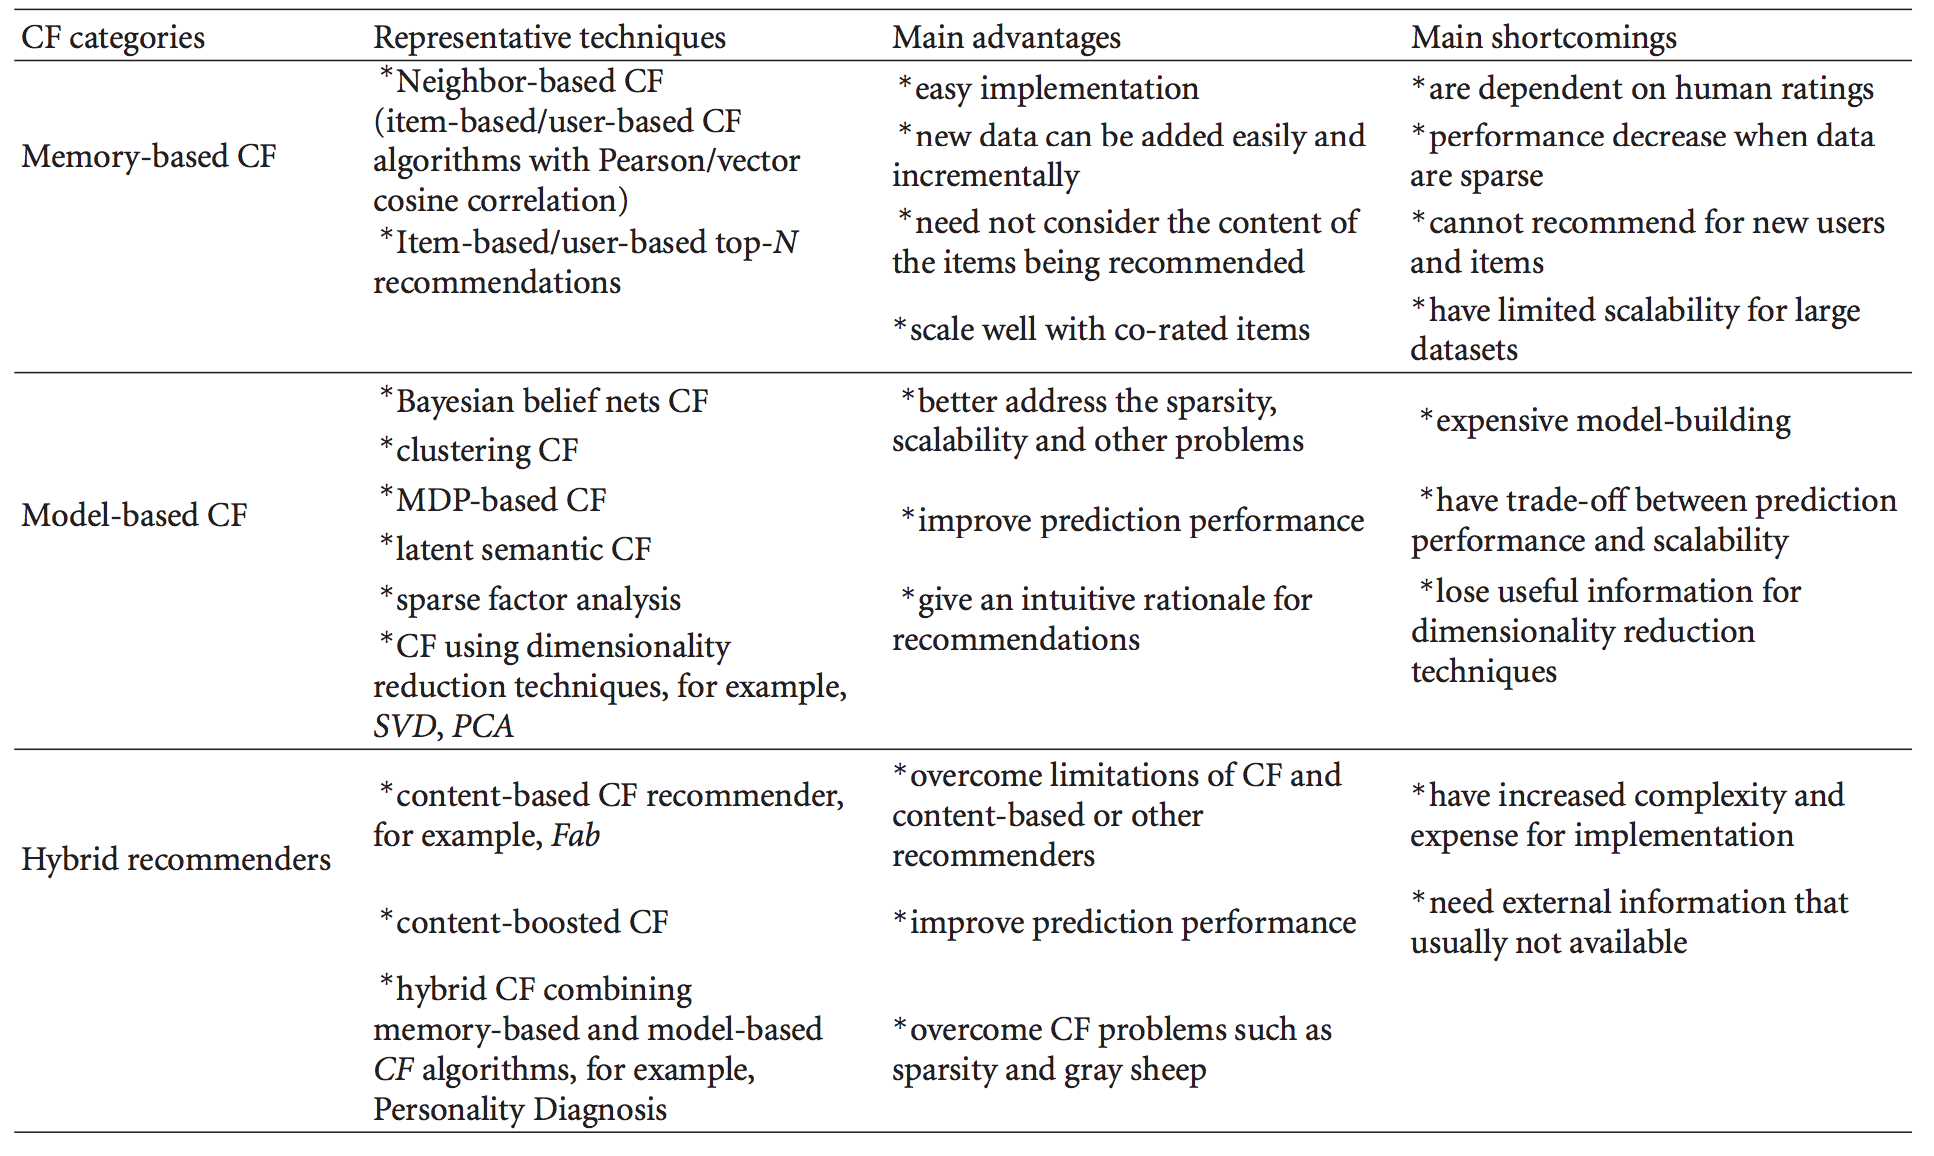
\includegraphics[width=35em]{cf-comparison}
    \end{center}
    \label{fig:cf-comparison}
    \legend{Source: \cite{Su2009}}
\end{figure}

\section{Content-based Filtering} \label{cb}
In this approach, a vector description of each item is constructed using structured data or some sort of item presentation algorithms such as Latent Dirichlet Allocation (LDA) or TF-IDF, which are used to build structured representations of unstructured data such as unrestricted text fields. Along with the item descriptions, a user profile is created for each user. This profile can consist of many different types of information: a history of the user's interaction with the system such as page views, searches and purchases is often used to train the model without any explicit user input. Some systems may require the user to explicitly state their interests, however it may be very hard to get users to make this effort, rendering this approach very limited in practice. Item representations and the user profile are then combined to create a model that, given a user profile and a new, unlabeled item, predicts the rating for the new item. One simple approach, for instance, would be a nearest neighbor method that calculates the distance between this new item and items already rated by the user and classifies this new item according to the labels of its nearest neighbors.

As CB filtering focuses on item rather than user similarity, it avoids the cold start problem since little information about user preference is needed. For instance, if user Bob rated movie $A$ but no other ratings are available for the movie, it is still possible to recommend other movies based on the attributes of movie $A$, such as genre keywords or release date. However, since only similar items to those already rated by the user will be considered, CB strategies tend to suffer from over-specialization \cite{Iaquinta2008}. This is known as the serendipity problem. Another limitation of CB algorithms is that items are required to contain enough information in order to distinguish items the user likes from items the user does not like. For example, a dataset of songs where only the song name is available would not be enough to make good predictions based on this content only, however this would pose no problem for collaborative filtering methods which rely solely on user similarity. Finally, while CB methods excel in recommending new items, they are not effective when it comes to new users. This is because the training model requires a rating history in order to make robust predictions.

CB systems provide several advantages over CF approaches:
\begin{itemize}
\item \emph{User independence}: CB systems do not rely on rating information from other users; this makes it possible to recommend items that were not yet rated by anyone else, based solely on the items characteristics. 
\item \emph{Transparency}: Predictions can be explained by listing specific content features that caused an item to be recommended.
\end{itemize}
On the other hand, several shortcomings are present when compared to CF approaches:
\begin{itemize}
\item \emph{User independence}: CB systems do not rely on rating information from other users, this makes it possible to recommend items that were not yet rated by anyone else, based solely on the items characteristics. 
\item \emph{Limited content analysis}: feature extraction is limited in most cases, limiting the amount of information available to build the user model. For instance, performing a text analysis on a news article will often completely ignore multimedia information
\item \emph{Over-specialization}: Also called the serendipity problem, CB systems are, by design, only able to recommend similar items to those already rated by the user. This makes it impossible for the user to discover novel and unexpected items.
\end{itemize}

In the next section, we provide a detailed explanation of Gradient Boosting Trees, which can be used as a binary classifier to implement a CB system by considering a positive rating as belonging to the positive class and a negative rating as belonging to the negative class.

\subsection{Gradient Boosting Trees}
In recent years, tree boosting has become an increasingly popular method and been shown to give state-of-the-art results for many classification problems \cite{Li2012} \bruno{algo errado com essa citacao; ta faltando o ano/mais dados no .bib?}. As in any supervised learning method, our objective is to train a model to predict a target variable $y_i$ given features $x_i$. Boosting methods are characterized by combining many weak learners into a strong one in an iterative fashion. In this case, the model is an ensemble of trees, more specifically a set of classification and regression trees (CART). Unlike decision trees, where the leafs contain decision values, the leafs on gradient boosting trees contain a score $s \in \mathbb{R}$. Multiple simple trees are then constructed and the prediction of each tree is summed up to get the final score as explained on Figure-~\ref{fig:ex1}. The model can then be defined as

$$\hat{y}_i = \sum_{k=1}^K f_k(x_i), f_k \in \mathcal{F}$$

\noindent where \(K\) is the number of trees, \(f\) is a function in the functional space $\mathcal{F}$, and $\mathcal{F}$ is the set of all possible CARTs \cite{Chen2016}. The example in Figure-~\ref{fig:ex1} tries to predict whether someone will like computer games or not. We can use the above equation to compute the score for the boy, for example, by summing the corresponding leaf scores of each tree \adriano{, i.e. the overall score associated with a given class is the sum of the scores (as predicted by each individual tree) for that class}.

\begin{figure}[ht!]
    \caption{GbTree example}
    \begin{center}
        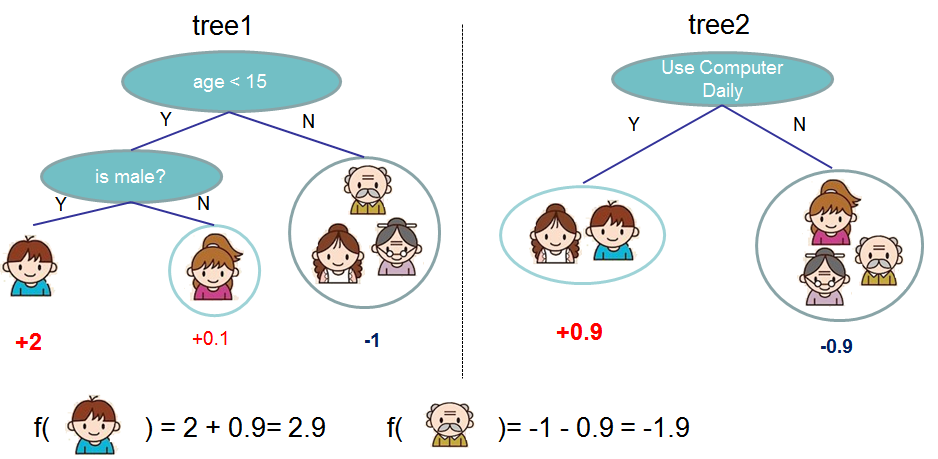
\includegraphics[width=28em]{twocart}
    \end{center}
    \legend{Source: XGBoost official site \bruno{colocar a citacao propriamente dita pro site.}} \pergunta{coloco o link aqui mesmo?} \bruno{nao o link, a citacao. Tem que ver como se faz citacao de site no padrao abnt}
    \label{fig:ex1}
\end{figure}

The objective function can be written as
$$\text{obj}(\theta) = L(\theta) + \Omega(\theta)$$
$$\text{obj}(\theta) = \sum_i^n l(y_i, \hat{y}_i) + \sum_{k=1}^K \Omega(f_k)$$

\noindent where $L$ is the training loss function and $\Omega$ is the regularization term. \adriano{$L$ can also be written as the sum of the errors for all instances given by an error function $l$ that takes as parameters the real class $y_i$ and the predicted class $\hat{y}_i$.}

One possible loss function would be the logistic loss function for logistic regression:

$$L(\theta) = \sum_i[ y_i\ln (1+e^{-\hat{y}_i}) + (1-y_i)\ln (1+e^{\hat{y}_i})]$$

To define the regularization function, we first define the tree function $f_t(x)$ \adriano{for each tree $t$} as
$$
f_t(x) = w_{q(x)}, w \in R^T, q:R^d\rightarrow \{1,2,\cdots,T\} .
$$
\noindent where w is the vector of scores on leaves \adriano{for some given input $x$}, $q$ is a function assigning each data point to the corresponding leaf, and T is the number of leaves. The regularization function is then defined as follows: \bruno{f é passado como parametro pra omega mas nunca usado?} \adriano{coloquei a definicao acima} \bruno{ainda nao entendi. A funcao $\Omega(f)$ nunca usa $f$ do lado direito da igualdade..} \adriano{$f$ é definido por $w$ que é usado do lado direito, coloquei na igualdade pra ficar mais claro}

$$\Omega(f) = \Omega(w_{q(x)}) = \gamma T + \frac{1}{2}\lambda \sum_{j=1}^T w_j^2$$


The ensemble is trained by using an additive strategy. We need to learn the functions $f$ that define the structure and leaf scores of each tree. This is done by fixing \adriano{the trees} we have already learned and, \adriano{based on them}, adding one new tree at a time. The prediction value at step $t$ ($t$-th tree) \adriano{for each instance $i$} is given by:

$$
\hat{y}_i^{(0)} = 0\\
$$
$$
\hat{y}_i^{(1)} = f_1(x_i) = \hat{y}_i^{(0)} + f_1(x_i)
$$
$$
\dots
$$
$$
\hat{y}_i^{(t)} = \sum_{k=1}^t f_k(x_i)= \hat{y}_i^{(t-1)} + f_t(x_i)
$$

We optimize the objective function \adriano{to build the tree at each step}: \bruno{como assim, 'choose'? Tu escolhe dentre N existentes? Ou tu quer dizer, pra treinar os parametros da $t$-th arvore? E porque precisa dessa outra funcao objetivo, se antes ja tinha a funcao objetivo $L$? e o que é $l$ minusculo usado na funcao $\mbox{obj}$?} \adriano{expliquei melhor $l$ no começo da secão}
$$
\text{obj}^{(t)} = \sum_{i=1}^n l(y_i, \hat{y}_i^{(t)}) + \sum_{i=1}^t\Omega(f_i)
$$
$$
= \sum_{i=1}^n l(y_i, \hat{y}_i^{(t-1)} + f_t(x_i)) + \Omega(f_t) + constant
$$

After some algebra, the objective becomes:
$$
\sum_{i=1}^n [g_i f_t(x_i) + \frac{1}{2} h_i f_t^2(x_i)] + \Omega(f_t)
$$
\noindent where $g_i = \partial_{\hat{y}_i^{(t-1)}} l(y_i, \hat{y}_i^{(t-1)})$ and $h_i = \partial_{\hat{y}_i^{(t-1)}}^2 l(y_i, \hat{y}_i^{(t-1)})$. By defining $G_j = \sum_{i\in I_j} g_i$ and $H_j = \sum_{i\in I_j} h_i$, \adriano{with $I_j = \{i|q(x_i)=j\}$ being the set of indices of data points assigned to the $j$-th leaf}, we can further simplify the objective function as:
$$
\text{obj}^\ast = -\frac{1}{2} \sum_{j=1}^T \frac{G_j^2}{H_j+\lambda} + \gamma T
$$

\bruno{TODO: parei aqui}
Finally, \adriano{by using this definition of the objective function,} we compute the score gain obtained by splitting a leaf into two leaves. The model is then trained by optimizing for one level of the tree at a time: \bruno{nao consegui entender qual a relacao entre a funcao objetivo anterior e essa ideia de usar o objetivo (generico) de regressao com regularizacao para treinar a arvore um nivel por vez. O algoritmo nao esta bem explicado..}
$$
Gain = \frac{1}{2} \left[\frac{G_L^2}{H_L+\lambda}+\frac{G_R^2}{H_R+\lambda}-\frac{(G_L+G_R)^2}{H_L+H_R+\lambda}\right] - \gamma
$$

\noindent \adriano{the gain can be decomposed as the sum of the new left and right leafs minus the score of the original leaf. We can see that if the gain is smaller than $\gamma$ we should not split the branch. This is the pruning step in the algorithm, after this, we can start building the next tree of the ensemble, up to the specified number of trees desired.}
\section{Hybrid systems}
When used in isolation, all the previous methods present shortcomings that are hard to overcome. Hybrid systems are often used to solve these shortcomings by combining results from many distinct models. There are basically 3 ways of creating hybrid systems:
\begin{itemize}
\item \emph{Ensemble design}: In this design, results from several algorithms are combined into a single output. This can be done in several ways, such as computing the weighted average of the various predictions or by multiplying every prediction. It's also possible to not directly combine the outputs, but instead, use the output from one algorithm as a feature for the next one.
\item \emph{Monolithic design}: In this approach, various data types are used as an input for a single generic algorithm. This can be done by, for example, modifying existing CB algorithms to take user rating matrices into account.
\item \emph{Mixed systems}: Like ensemble design, the output from multiple algorithms is computed to obtain a score for each item, however, instead of combining these scores, items from each algorithm are presented together side-by-side.
\end{itemize}

We can formalize the weighted average method \adriano{from the ensemble design}, which will be used in this work, by defining $R = [r_{uj}]$ as a $m \times n$ matrix of completely specified ratings, in which the unobserved entries of $R$ are predicted by $q$ different algorithms. For a set of weights $\alpha_1 .. \alpha_q$, the weighted hybrid method creates a combined prediction $\hat{R}$ as follows:
$$
\hat{R} = \sum_{i=1}^{q}{\alpha_i\hat{R_i}}
$$

Linear regression can be used to determine the optimal weights by minimizing metrics such as the \emph{MSE} or \emph{MAE}.


\chapter{Experimental Methodology} \label{experiment}

\bruno{tem que ter um paragrafo de introducao explicando mais detalhes do que ta acontecendo. O capto comecou direto listando variaveis que tem dentro do teu modelo, sem antes definir ou explicar, p.ex., o que é o 'experimento' que tu menciona na 1a frase. O experimento é um só? Ou é um conjunto de experimentos comparando N algoritmos dentre os mencinados no capto anterior? Precisa explicar, tipo 'Dentre os N algoritmos anteriores, selecionamos para avaliacao os algoritmo A1, A2 e A3. Nosso objetivo nas proximas secoes será aplicar e comparar quantitativamente e qualitativemente a performance desses algoritmos quando usados para criar um SR para o Catarse. Para isso, iremos, inicialmente, descrever a metodologia que será utilizada nesses experimentos comparativos. Em particular, iremos descrever quais sao os dados de treinamento que estao disponiveis no sistema para o qual iremos criar um SR, como essas dados sao preparados antes da utilizacao dos algoritmos de treinamento, e tambem as metricas de performance que sera utilizadas a fim de avaliar a performance relativa de cada abordagem'. Coisas desse tipo é que precisam ir no paragrafo de introducao, senao o leitor começa a ler e nao tem ideia de que experimento tu ta falando, do que tu vai fazer, o que tu vai comparar, quais algoritmos tu escolheu, POR QUE tu escolheu esses algoritmos. Tudo isso precisa ser explicado e discutido} \adriano{feito abaixo}

\adriano{Our experiment consisted of implementing and evaluating three recommendation algorithms using data available in Catarse's database. The chosen algorithms were: Collaborative Filtering with matrix factorization, a Content-Based approach using Gradient Boosting Trees, and a Hybrid system combining these two methods by using weighted averages. These algorithms were chosen due to their state-of-the-art performance and wide use in the industry, and also to test every major approach in RSs in the context of Catarse's environment. The existing popularity ranking was used as a baseline in our tests.}

\adriano{In the next few sections, we will describe how our training data was obtained and prepared for use in each RS implementation, as well as provide evaluation metrics that are commonly used in recommender systems in order to compare each approach. The main benefits and shortcomings of each metric will be presented and their applicability to our experiment will also be discussed.}

\section{Data Preparation} \label{data-preparation}
\adriano{Two datasets were constructed from Catarses's production database: one for our CB model and one for the CF model}. Each example in the dataset \(D\) for our CB model consists of a project-backer pair \((p,b)\) with 12 dimensions presented below:
\begin{itemize}

    \item \emph{category count}: Number of projects backed by the user \(b\) in the same category as project \(p\);
    \item \emph{mode count}: Number of projects backed by the user \(b\) with the same \adriano{funding mode} (\adriano{all-or-nothing, flexible or subscription}) as project \(p\);
    \item \emph{same state}: True if the project \adriano{geographic} location is the same as the backer's;
    \item \emph{recommended}: True if project \(p\) was manually recommended by an admin;
    \item \emph{has video}: True if the project\adriano{'s creator} has uploaded a video \adriano{describing it};
    \item \emph{budget}: \adriano{Length of the textual description (prepared by the project's creator) of the project's budget;}
    \item \emph{description}: \adriano{Length of the textual description (prepared by the project's creator) of the project's description;}
    \item \emph{pledged}: Amount pledged in the first 3 days \adriano{since the launch of the project;}
    \item \emph{contributions}: Amount of contributions in the first 3 days
    \item \emph{progress}: Percentage of goal reached in the first 3 days \adriano{since the launch of the project;}
    \item \emph{owner projects}: Amount of projects from the same project owner as \(p\);
    \item \emph{reward count}: Number of offered rewards in project \(p\);
\end{itemize}

In order to trim irrelevant data, we remove canceled and draft projects as well as projects with no backers from the dataset. The final cardinality of \(D\) was 300000 \adriano{$(p,b)$ pairs}. \adriano{Since $D$ consisted of only positive samples (a user backing a project denotes a positive action),} for the sake of balancing our dataset, we create 300000 more negative instances by randomly combining users with projects they haven't backed \bruno{dizer qual eram os percentuais de classes antes de tu fazer isso} \adriano{explicado acima}. To further emphasize project quality, only successful projects are considered for the positive instances, while only failed projects are used for the negative instances \bruno{fail e success according to what?} \pergunta{acho melhor explicar essas definicoes numa secao separada ne?}. Finally, due to changes in the platform that occurred in 2015, we ignore data from earlier periods so as to maintain a consistent dataset.

The dataset used for the Collaborative Filtering model is a simple list of User ID and Project ID pairs \bruno{ta, tu ta usando CF tambem. Entao no inicio da secao tem que dizer que tu avaliar algoritmos representativos das duas classes de approaches, e que tu vai, a seguir, explicar como tu preparou os dados de treinamento pra cada uma delas} \adriano{explicado acima}, one for each contribution in the database. With this information, we build a \(R_{n\times m}\) matrix where $N$ is the number of users and $M$ the number of projects. The rows indices represent the User ID, while the columns indexes represent the Project ID. A specific entry $R_{i,j}$ will be $1$ if there exists a contribution made by the user with ID $i$ to project with ID $j$, and $0$ otherwise. At the time of writing, the cardinality of $N$ was 900k and $M$ was 75k, resulting in a matrix $R$ with 67.5 billion entries. To achieve reasonable memory consumption, $R$ is converted to a sparse representation.

\section{Evaluation Metrics} \label{metrics}
There are basically 3 ways RSs can be evaluated: offline, online, and empirically. Offline measures are those computed based on a given static dataset, generally through techniques such as split validation and cross-validation. In these techniques, a subset of the data is withheld to be later used for testing; metrics are then computed for the test set only. According to Herlocker et al. \cite{Herlocker2004}, offline metrics can be broadly classified into the following categories: predictive accuracy metrics, such as Mean Absolute Error (MAE) and its variations; classification accuracy metrics, such as precision, recall and F1-measure; rank accuracy metrics, such as Pearson’s product-moment correlation, and normalized distance-based performance metric (NDPM). To define precision and recall, which will be used to measure performance in this work, we must first define the following terms: True Positives (\textbf{TP}): number of instances classified as belonging to its true class; True Negatives (\textbf{TN}): number of instances classified as not belonging to class A and that in fact do not belong to class A; False Positives (\textbf{FP}): number of instances classified as class A but that do not belong to class A; False Negatives (\textbf{FN}): instances not classified as belonging to class v but that in fact do belong to class A. We can then define precision as $P = T P/(T P + F P)$, recall as $R = TP/(TP+FN)$ and accuracy as $A = TP + TN/(TP+TN+FP+FN)$.

\adriano{For ranked recommendations, we also define the Recall@N metric which evaluates whether an item the user has rated in the past is in the top N recommendations from a random set of projects. It works as follows: a set of 100 random projects is augmented with a project the user has interacted previously, we then measure if the interacted project is present in the top N recommendations.}

\adriano{In the experiments discussed in chapter \ref{results}}, we will present \adriano{results for some of }these offline metrics for each implemented algorithm; however, it should be noted that they are not good indicators as to how well a RS will actually perform \adriano{in production}, and trying to optimize for them may actually degrade real-life performance \cite{McNee2006}. To illustrate this point, let's think about a recommender system for movies. Suppose user Bob likes movies $A$, $B$ and $C$. We split our dataset in such a way that movies $A$ and $B$ will be in the train set, while movie $C$ is on the test set. Any kind of offline metric will test in a way or another if movie $C$ was recommended to user Bob, resulting in a higher score if it is recommended and a lower score if other, unrelated movies, are recommended. The problem is that an algorithm that recommends movies $D$ or $E$ could actually be much better than one that recommends movie $C$, a fact that no offline metric could account for. This can be fundamentally attributed to the fact that, unlike most classification problems, recommender systems work with extremely sparse matrices; this sort of validation strategy would only be valid if we knew the ratings given by the user for every item beforehand. Evidently, in this imaginary scenario a RS would be pointless in the first place, consequently, other evaluation strategies are required.

Much more meaningful metrics can be obtained by online evaluation. While much more expensive and time-consuming to perform than offline measurements, live metrics are capable of testing directly whether the RS is achieving its intended purpose. The most common measures are the Click-Through Rate (CTR) and Conversion Rate (CR). CTR is defined as the ratio of users who click on a specific link \adriano{with respect} to the number of users who viewed the page. In our case, if a set of $N$ recommendations is displayed $X$ times \adriano{for distinct users} \bruno{cada recomendacao é exibida X vezes pra um mesmo usuario?}, let $Y$ be the number of times a user clicked on at least one of the recommended items in $N$. CTR is then defined as $\frac{Y}{X}$. \adriano{CR is defined in the same way as CTR, except that users most not only click on a specific recommendation but also back the project} \bruno{porque?} \adriano{reescrevi para ficar mais claro}. To compare two different RSs in an online setting, the most prominent approach today is A/B-testing. Since our experiment consists of 3 different approaches \bruno{isso nunca foi explicado antes. Quais 3 approaches? precisa explicar isso no inicio} \adriano{feito}, an A/B/C test will be performed. For our \adriano{online} experiment, a recommendation algorithm was randomly selected for each user and click-through and conversion rates were measured by adding a reference header to projects that were accessed through the recommendations page.\bruno{selecionar 1 algoritmo por usuario funciona caso o alg. seja user-based, mas e se for desses algoritmos que aprendem padroes nao so pra um usuario, mas relacionam todos usuarios com todos os itens?} \adriano{todos os algoritmos sao treinados com dados de todos usuarios e projetos, mas para fazer a predicao recebem apenas um usuario e projeto (usando esse modelo ja treinado). vou tentar deixar isso mais claro no referencial teorico }

Finally, empirical evaluation consists in having a person actually look at the results \bruno{quais results? recomendacoes? pra um usuario especifico? pra varios?} \adriano{for one or more user profiles}. This is equally important in any business setting. Consider a news portal that implemented a RS for its front page news. The RS might start recommending articles about cute cats, which might very well provide higher click-through rates than its more serious articles. This, however, is probably not what the company had in mind, and such a change in content might hurt the company's reputation in the long run. It is thus paramount to perform sanity checks on recommendation results manually. To achieve this, a test page with each proposed algorithm was made available and a survey was sent to 14 members of the Catarse team. The following questions were asked about each algorithm:

\begin{enumerate}
    \item: What is your level of satisfaction with this algorithm?
    \item: How would you classify this algorithm with respect to the following properties (5 ratings, ranging from very unsatisfied to very satisfied)?
    \begin {itemize}
    \item: This algorithm showed me projects I would back \bruno{os items 2.1-2.3 (alias, tem que corrigir a numeracao abaixo) sao subitens do no.2? Nao parecem ser. Parecem nem ser coisas mutuamente exclusivas. Also, se tu quiser numeracao, nao precisa fazer um itemize com numeros digitados manualmente em cada item. Existe um comando chamado enumerate, que faz isso (usar ao inves do itemize)} \adriano{na verdade sao subitens, ja que a segunda pergunta pede para dar uma nota de 1 a 5 para cada caracteristica. mudei para enumerate no primeiro nivel das perguntas}
    \item: This algorithm showed me projects I didn't know about
    \item: This algorithm positively surprised me 
    \end{itemize}
\end{enumerate}

%% \begin{figure}
%%     \caption{Feature weights in gbtree}
%%     \begin{center}
%%         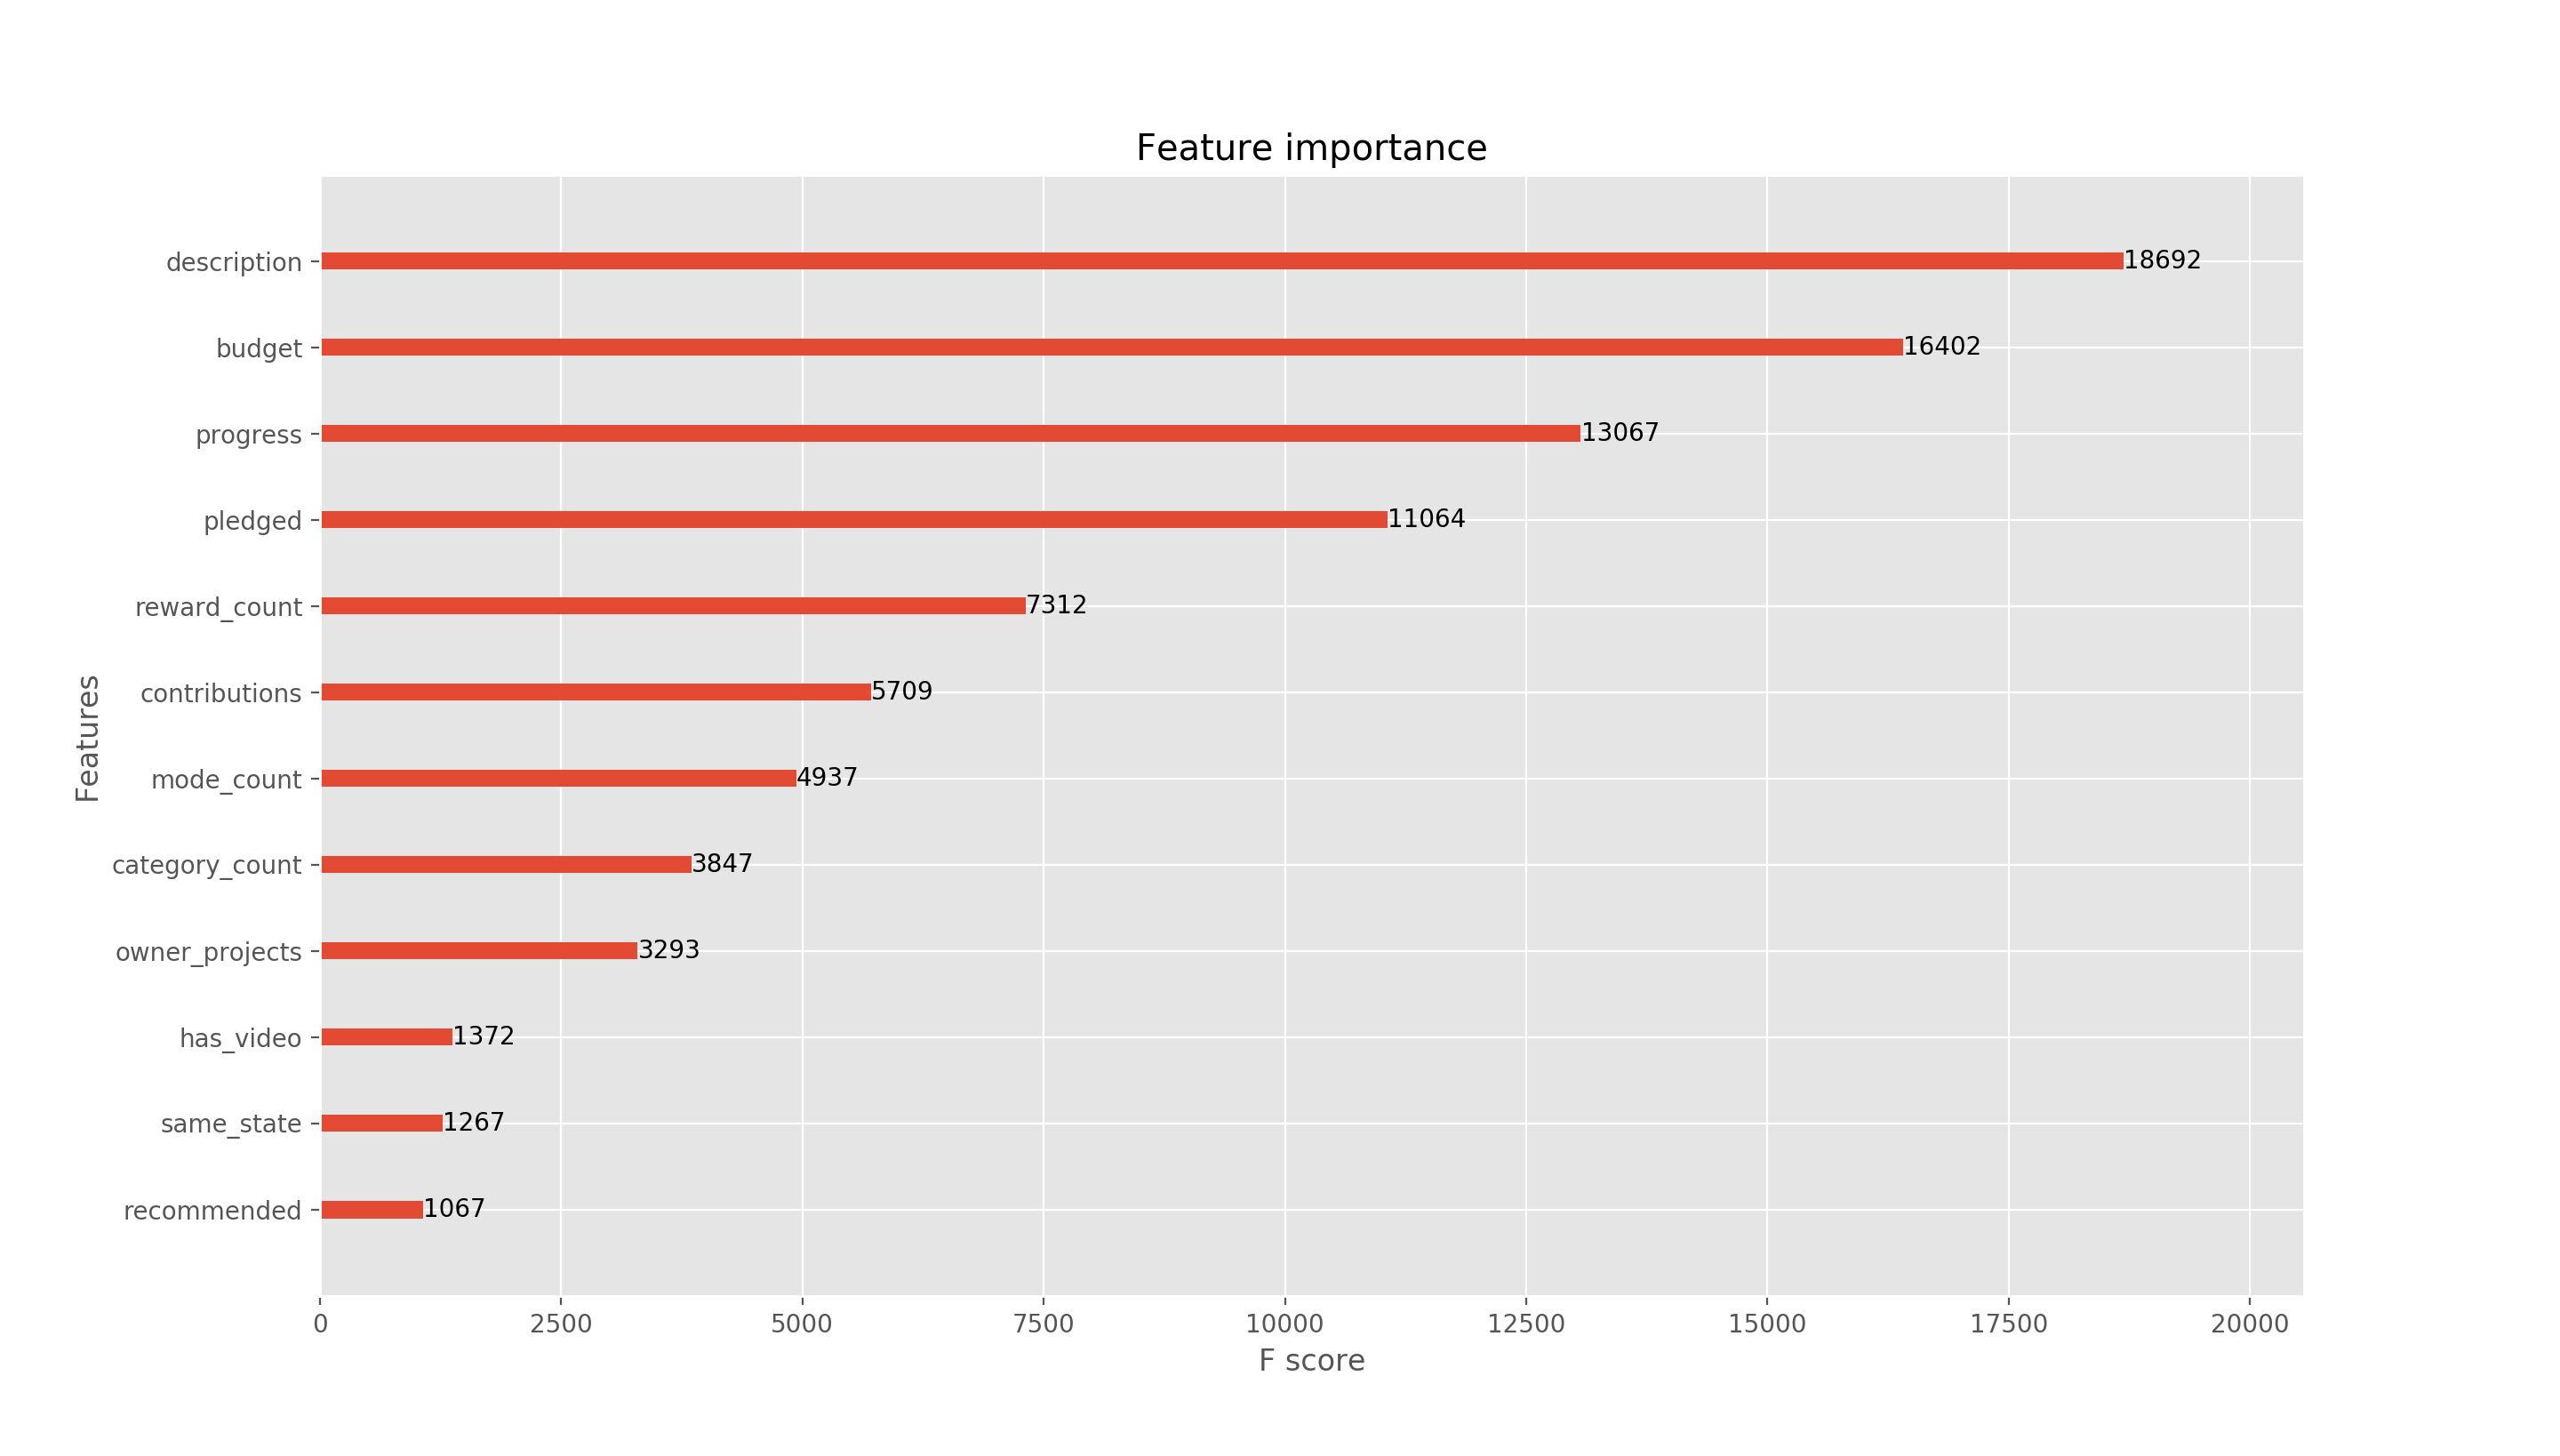
\includegraphics[width=35em]{featureweights}
%%     \end{center}
%%     \label{fig:features}
%% \end{figure}

%% Collaborative filtering train AUC: 0.9910468
%% Collaborative filtering test AUC: 0.9863695
%% Collaborative filtering test precision: 0.010246708
%% Collaborative filtering test recall: 0.08933075888822199


\chapter{Results} \label{results}
In this chapter, we give results \adriano{for our three implemented algorithms} according to the offline, online, and empirical metrics. The computed offline metrics were accuracy, recall, and precision, \adriano{as defined on section \ref{metrics}}.

\section{\adriano{A Content-Based RS for Catarse}}
\adriano{The Gradient Boosting tree method was chosen for our Content-Based system due to its state-of-the-art performance in many real-world applications \cite{Chen2016}. The data described in section \ref{data-preparation} was used to train a model that predicts the backing probability of any user-project pair.} The XGBoost python library was used for this implementation. Hyperparameters were tuned by running 10-fold cross validation while optimizing for negative log-likelihood. No data standardization or normalization was necessary since the base learners are trees. In order to understand how each feature affects the outcome prediction in our model, we plot the SHAP \footnote{SHAP is a unified approach to explain the output of any machine learning model. SHAP connects game theory with local explanations, uniting several previous methods and representing the only possible consistent and locally accurate additive feature attribution method based on expectations. \cite{Lundberg2017}} values of every feature for every sample in figure ~\ref{fig:features_importance}. From this plot, we can draw some interesting conclusions: the most important feature in determining backing probability \bruno{tu nao explicou que o que o modelo vai prever é backing probability. Antes tu tava falando de prever os top-k projetos no ranking, coisas desse tipo} \adriano{explicado acima} is the number of backed projects in the same category, followed closely by the project progress in the first 3 days. We can also see that having a low number of available rewards decreases backing probability.

\begin{figure}[ht!]
    \caption{Feature importance in Gradient Boosting Tree}
    \begin{center}
        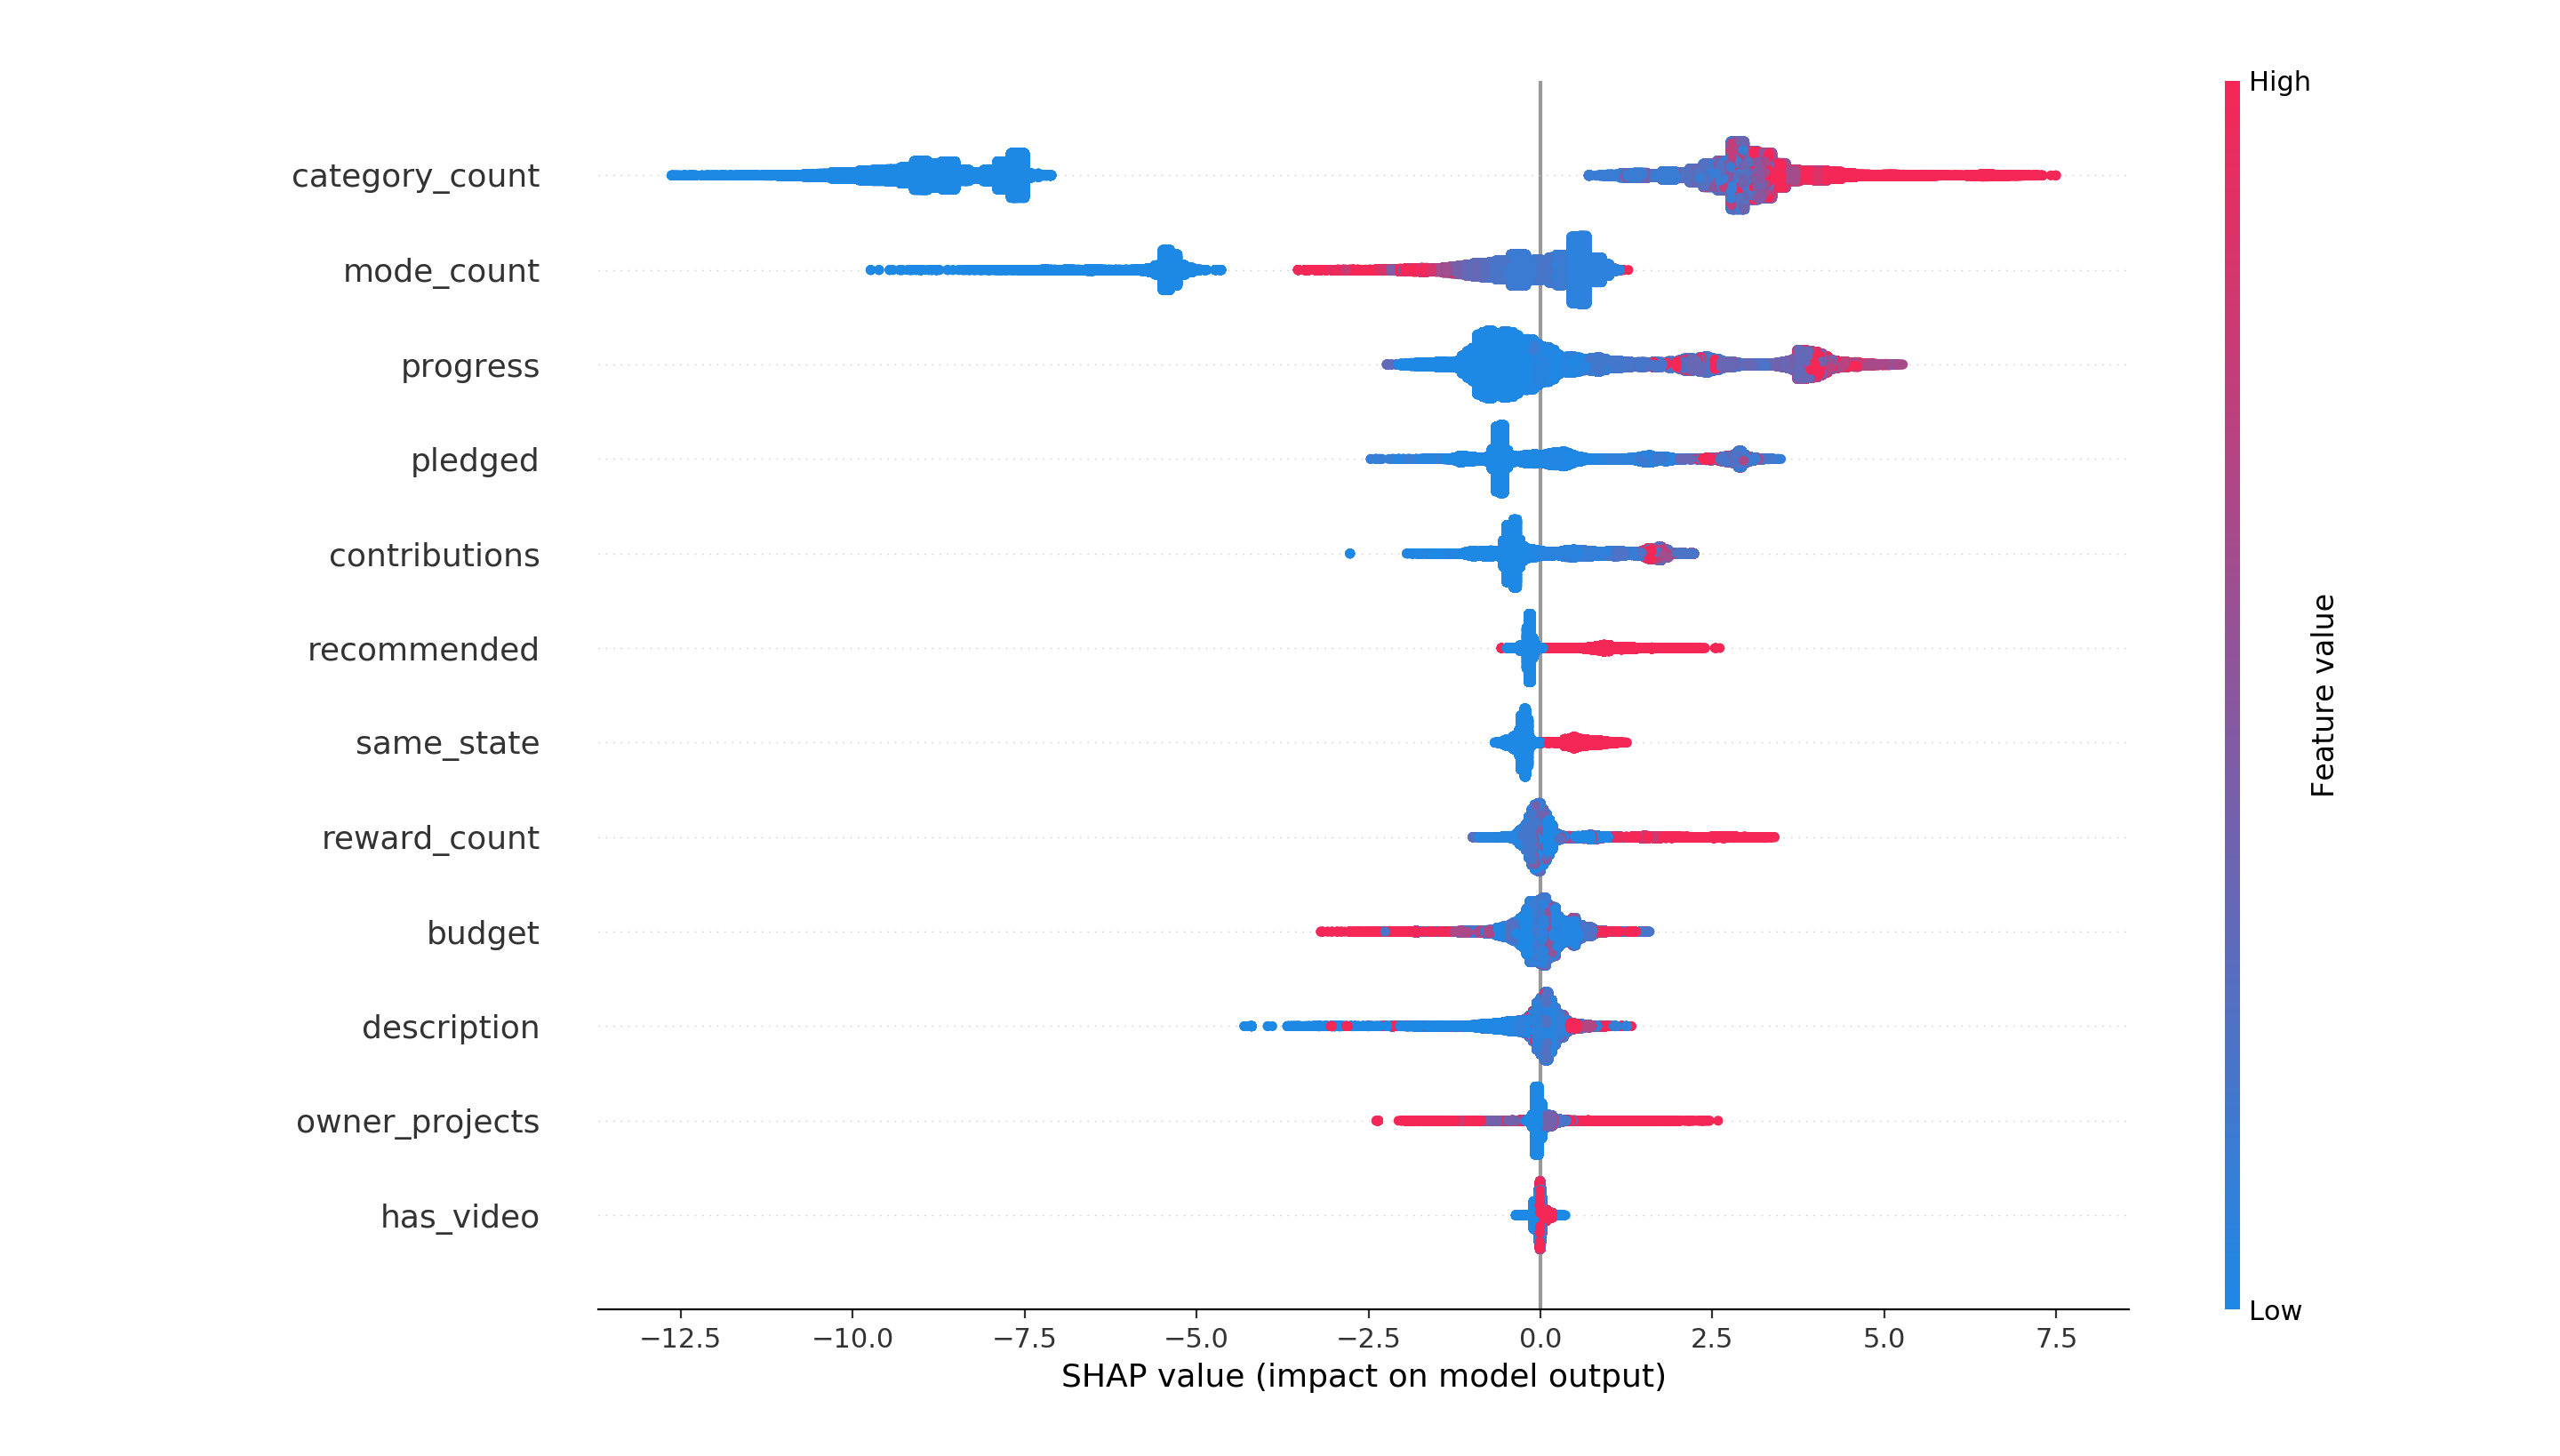
\includegraphics[width=\textwidth]{feature_contribution}
    \end{center}
    \label{fig:features_importance}
\end{figure}

To determine how individual features affect the output of the model, let's take our most significant feature, $category\_count$, and plot its value against the corresponding SHAP value for all examples in our dataset. Vertical dispersion shows the interaction between features, in this case how $category\_count$ relates to $reward\_count$. The result is shown in figure ~\ref{fig:category_count}.

This approach gave exceptional results in every computed offline metric, as seen on table- ~\ref{tbl:cb_offline_metrics}. This, however, should be considered with care: our dataset is intrinsically predictable to the point that any method should give great results; in fact, a simple test to check if the $category\_count$ feature is greater than zero already yields us an accuracy of $94.5\%$. This is due to the fact that most users only back one project in one category.

\begin{table}[ht!]
    \caption{Content-Based Offline metrics \bruno{arrumar centralizacao}}
    \centering
        \begin{tabular}{c|c|p{5cm}}
          \hline
          \textit{Recall}  &   \textit{Accuracy}  &   \textit{Precision} \\
          \hline
          \hline
          0.990450           & 0.986260 &  0.982813 \\
          \hline
        \end{tabular}
    \label{tbl:cb_offline_metrics}
\end{table}

\begin{figure}[ht!]
    \caption{Dependence plot for category\_count \bruno{nao é claro o que esse grafico esta mostrando}}
    \begin{center}
        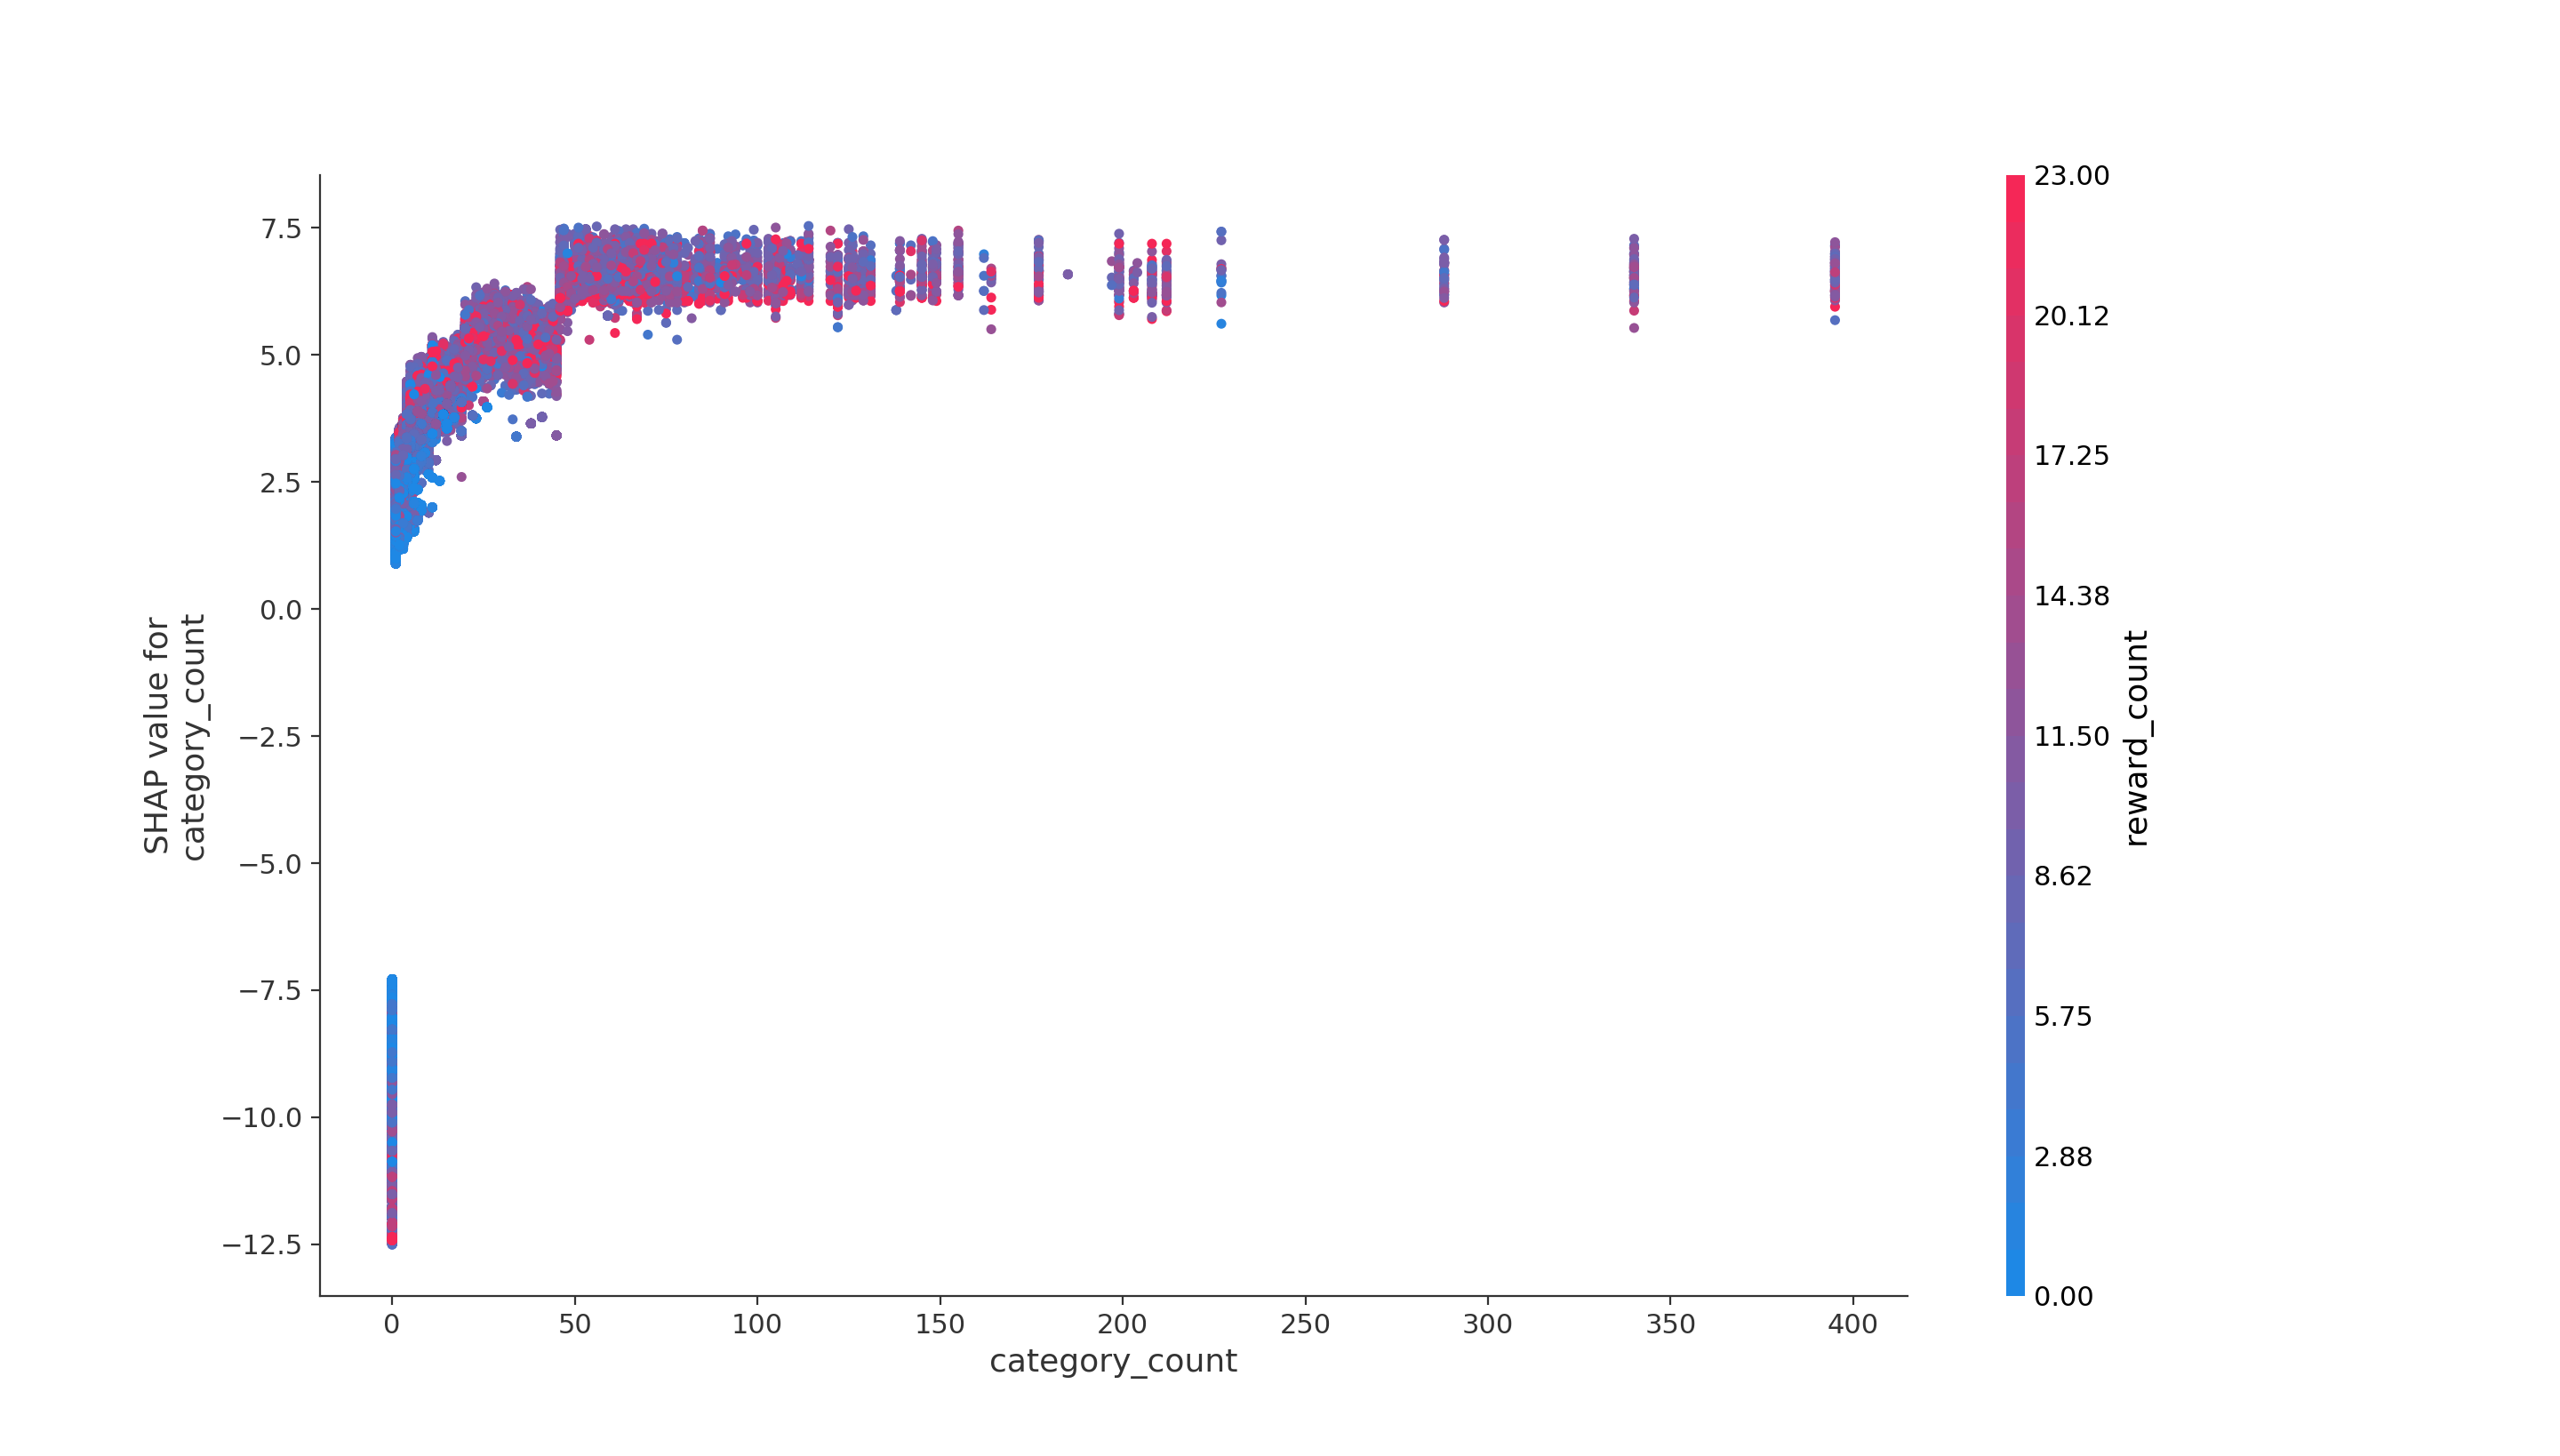
\includegraphics[width=\textwidth]{category_count}
    \end{center}
    \label{fig:category_count}
\end{figure}

\section{A Collaborative Filtering RS for Catarse}
Our Collaborative Filtering model was implemented using the LightFM library, \adriano{which uses a Model-based matrix factorization algorithm. This algorithm was chosen for its simplicity and high performance in our extremely sparse rating matrix (approximately 1 rating for every 75k entries in the matrix).} \bruno{qual dos sub-tipos de CF tu ta usando? relacionar com as varias variantes que foram descritas no capto de background teorico e explicar/justificar por que tu escolheu esse algoritmo especifico para a tua aplicacao. Por que nao outros? Quais as vantagens e desvantagens (como descrito naquela tabela comparativa) te levaram a essa escolha?}. As depicted on table-~\ref{tbl:cf_offline_metrics}, every offline metric \adriano{for the CF approach, applied to the Catarse system,} performed much worse than its Content-Based counterpart. This was expected due to our dataset characteristics: since most users only back one project in their lifetime there is not enough rating data for CF to perform well. However, \adriano{empirical and online tests (see sections \ref{empirical-evaluation} and \ref{online-evaluation})} using \adriano{the learned CF model} with real users provided much better results \bruno{onde esses resultados sao descritos? dizer aqui, porque o proximo paragrafo aparentemente nao comenta eles; tu menciona que tem resultados melhores mas ai nao fala mais nada sobre isso, nesse ponto do texto, e muda de assunto}. \adriano{coloquei referencias para as secoes onde estao os resultados}

Calculating \adriano{offline} metrics poses a problem for CF algorithms that produce ranked recommendations. \adriano{Given a user and a list of projects of size $N$, our model maps each project in the list to a real number and returns another list of size $N$ with these numbers, which can later be sorted to show the most relevant recommendations in order. These numbers can assume arbitrary values which have no relation to the backing probability; they are used for ranking purposes only.} \bruno{se eles sao usados pra ranking, eles TEM um significado. Talvez o que tu queira dizer é que o valor numerico especifico nao necessariamente corresponde à probabilidade real de backing, e sim apenas a uma indicacao RELATIVA de quao mais provavel é que um projeto especifico seja backed em relacao a outros projetos. Explicar um pouco mais cuidadosamente essa tua ultima frase} \adriano{acho que agora ficou mais claro} Therefore it is impossible to compute an error metric since we do note have two sets of comparable values to test for equality. However, \adriano{our hybrid approach requires that we have pairs of comparable numbers in order to compute the weighted average between CF and CB results. To make the CF model output comparable to our CB model output, which returns backing probability in the 0--1 range, we normalize the CF model output so it also stays in the 0--1 range. We then consider any normalized value greater than $0.5$ to be in the positive class, and negative otherwise. These classes derived from the normalized values can then be used to compute offline metrics for our CF model. This gives us an accuracy of approximately $93\%$, or equivalently an error of $7\%$.}  \bruno{por que é possivel na abordagem hibrida? Alias, tu nunca falou, antes, que iria testar uma hibrida, eu acho. Ela é a combinacao de que? Precisa explicar isso quanto tu fala e motiva/justifica os N algoritmos que tu vai comparar nos experimentos} \pergunta{isso eh meio que uma gambiarra pq na verdade essas metricas(ainda nao estao na tabela, vou colocar depois) nao fazem sentido pro modelo em si, mas eu preferi apresenta-las para ter um modo de comparar o resultado do CB com o CF. nao sei se isso foi uma boa ideia ou se eh melhor simplesmente dizer que isso eh impossivel e deixar por assim mesmo}


\begin{table}[ht!]
    \caption{Collaborative Filtering Offline metrics \bruno{que que é o recall@x? Explicar no texto o que é o 'x'.} \adriano{coloquei no capitulo de metricas}}
    \centering
        \begin{tabular}{c|c|c|p{5cm}}
          \hline
          \textit{Recall@5}  &   \textit{Recall@10}  &   \textit{Precision@5} &   \textit{Precision@10} \\
          \hline
          \hline
          0.06500372900657606           & 0.0925860086205232 &  0.015118373  & 0.010974493  \\
          \hline
        \end{tabular}
    \label{tbl:cf_offline_metrics}
\end{table}

\section{A Hybrid RS for Catarse}
Hybrid ratings were computed by taking the weighted average of the ratings obtained by the CB method and the normalized CF ratings \bruno{isso precisa ser descrito antes, pra que quando tu comecar a falar dos experimentos que serao feitos, tu diga pro leitor QUAIS vao ser os experimentos: vai ser com o alg1 da abordagem CF, alg2 da abordagem CB, e alg3 hibrido combinando metodos A e B; e que cada um desses sera avaliado de acordo com as 3 metricos (X,Y,Z) descritas na secao de metodologia}. \adriano{feito} By doing this, we hope to compensate any weaknesses in the original techniques and leverage its strengths. For example, a project highly rated by our CB algorithm but rated lowly by the CF algorithm could show that, although its features seem to indicate a good match for the user, similar users are not backing it in practice. By averaging both ratings such a project would rank much lower on the recommendation list, allowing better matching projects to appear in higher positions.

\section{Comparison of CB, CF, and Hybrid (offline metrics)}
\bruno{essa secao tá só mostrando os valores das tabelas anteriores, todos juntos? Ou tem algo diferente?} \adriano{TODO: discutir resultados}

Table \ref{tbl:offline_metrics} summarizes offline results for our three tested approaches. 

\begin{table}[ht!]
    \caption{Offline metrics}
    % OBS: não use \begin{center}, pois este aumenta o espaçamento entre a caption/legend e a tabela
    % Para figuras, a aparência é melhor com o espaçamento extra
    \centering
        \begin{tabular}{c|c|c|p{5cm}}
          \hline
          \textit{Method}  &   \textit{Recall}  &   \textit{Accuracy}  &   \textit{Precision} \\
          \hline
          \hline
          Content-Based           &   0.990450           & 0.986260 &  0.982813 \\
          Collaborative Filtering     & 0.089330             & 0.932910  & 0.010246\\
          Hybrid     & 0.942722             & 0.964293  & 0.928434\\
          \hline
        \end{tabular}`
    \label{tbl:offline_metrics}
\end{table}

\section{Comparison of CB, CF, and Hybrid (online metrics)} \label{online-evaluation}
Online results were obtained by randomly assigning a recommendation algorithm for each user that visited the Explore Projects page. \adriano{The existing popularity metric was also added as a baseline for comparison, thus resulting in 4 test groups: CB, CF, Hybrid and popular. For each group CTR and CR measurements were obtained.} The experiment was run for 1 week on a live production environment with more than 20 thousand unique visitors per day.

It is known that the chance of obtaining a false positive increases with the number of variations tested. This probability is given by the formula $1-(1-a)^m$, with $m$ being the total number of variations tested and $a$ being the significance level, which gives us a false positive probability of $18\%$ when $m=4$ and $a=0.05$. To correct for this, we compute a new required confidence level by applying the Bonferroni correction, which calculates the confidence level for a test with more than one variation. This correction simply divides our desired significance level by the number of variations,  thus giving us a new required significance of $\frac{0.05}{4}=0.0125$, or, equivalently, a required confidence level of $98.75\%$. \bruno{mas cade os resultados do online? tu nao tinha dito que iria medir CTR e CR? Aonde tao esses valores?} \adriano{experimento terminou agora, coloquei os resultados abaixo}

\adriano{The measurements obtained are described in table-\ref{online-results}. We can see from these results that Click-Through rates only improved for the CF algorithm in comparison to our popular control group, while every other algorithm performed worse than baseline. One possible cause for this is the intrinsic recommendation diversity provided by the CF approach; both CB and Hybrid recommendations are more likely to show projects similar to those already backed by the user, for example, a user that usually backs comic books projects would be shown mostly projects about comic books. However, such a user probably has already seen most available comic books projects and is, therefore, less likely to click on them again. On the other hand, diverse recommendations provided by the CF approach will present novel projects which are more likely to be clicked on. Nonetheless, simply improving CTR does not necessarily increase Conversion Rate, which is our real objective; in fact, our CR results show a quite different picture: not only every recommendation approach performed significantly better than the baseline, but CF showed the least improvement while the Hybrid algorithm exhibited the best results, as was expected. In fact, almost half of project views from the Hybrid ranking resulted in pledges to the project, a particularly impressive result. The high amount of traffic gives us the required confidence level thus validating the results.}

\begin{table}[ht!]
\centering
\caption{Online results}
\label{online-results}
\begin{tabular}{|l|l|l|l|l|}
\hline
    & CF & CB & Hybrid & Popular \\ \hline
CTR \% & 42 & 34 & 33     & 38      \\ \hline
CR \% & 12 & 13 & 15     & 10      \\ \hline
\end{tabular}
\end{table}

\adriano{As discussed on chapter \ref{motivation}, our two main goals from the business perspective were to increase the amount of money pledged to projects and to increase the percentage of successful projects. The first goal seems to have been achieved when looking at our conversion rates: our hybrid approach resulted in 50\% more pledges than the existing popularity ranking. Our second goal, however, cannot be measured directly on such a short experiment, therefore an indirect metric is required for our comparison. It is reasonable to assume that more projects would be successful if pledges were distributed evenly among many projects instead of concentrating on just the most popular ones. Accordingly, we will measure the success of our second objective by looking at the project distribution of the pledges. The approach with the highest number of distinct projects pledged to will most likely meet our second goal. Table \ref{distinct-projects} show this analysis. We can see every implemented algorithm increased this metric, with the CF approach being the clear winner. Again, this can be explained by the diversity of results that is inherent to this approach.}

\adriano{From these results, it is clear that the CF and Hybrid approaches maximize different objectives. This creates an optimization problem that is business specific and beyond the scope of this work, but it is easy to see that this can be optimized by simply adjusting the weights in our Hybrid algorithm, giving more or less emphasis to the CF model.}

\begin{table}[ht!]
\centering
\caption{Number of distinct projects who received pledges}
\label{distinct-projects}
\begin{tabular}{|l|l|l|l|l|}
\hline
                   & CF & CB & Hybrid & Popular \\ \hline
Number of projects & 45 & 29 & 26     & 24      \\ \hline
\end{tabular}
\end{table}

\section{Comparison of CB, CF, and Hybrid (Empirical Evaluation) \bruno{essa é a expressao que normalmente se usa? empirical sugere uma coisa que tu rodou no sistema real (online), nao algo que foi baseada em opiniao subjetiva de especialistas. Talvez 'Human expert evaluation' ou algo assim?}} \adriano{em varios artigos que eu li foi usada essa expressao, e foi rodado em um sistema real sim, foi tipo uma avaliacao do sistema real subjetiva. vou deixar mais claro no texto abaixo} \label{empirical-evaluation}

\bruno{os resultados de online aparecem depois dos de empirical, o que é um pouco confuso porque tu disse, na explicacao, que iria testar offline, online, e empirical. Quando eu vi tu mostrando offline e empirical, eu pensei que de repente tu nao iria mostrar o online por alguma razao. Tenta ser consistente no sentido em que a ordem das secoes é a mesma ordem que tu menciona quando descreve as coisas que serao feitas. Isso vale pro resto do texto tambem} \adriano{movi o online para cima}

The results on table-~\ref{tbl:survey-results} were obtained by sending a survey to each member of Catarse's team. Respondents were asked to \adriano{evaluate} each available algorithm while logged in with their accounts \adriano{in a production environment} and answer several questions about each of them. To avoid bias, respondents were not given any details about the algorithms, which were labeled simply as 1, 2 and 3 to avoid identification. Five ratings were available for each question, from very unsatisfied to very satisfied. These rating were mapped to a 1-5 scale in order to obtain an average rating for each proposed question. It must be noted that, although this survey was aimed at people with vast knowledge and experience about crowdfunding projects, their recommendation results do not necessarily match those of a regular user. This is due to the fact that most site admins have backed hundreds of projects in order to test new features or while trying to reproduce bugs, which could greatly skew results since those projects are not necessarily the kind of projects they would normally back. To remove these outliers, only survey results of users with less than a 100 contributions \bruno{acho que 'contributions' nao foi definido; 1 contribution=1 pagto pra back 1 projeto especifico? precisa definir la no inicio, quando tu fala de alguns dos termos relacionados ao Catarse} were considered. 
\begin{table}[ht!]
\centering
\caption{Survey Results}
\label{tbl:survey-results}
\begin{tabular}{llll}
\hline
\multicolumn{1}{|l|}{}                                                        & \multicolumn{1}{l|}{CF} & \multicolumn{1}{l|}{CB} & \multicolumn{1}{l|}{Hybrid} \\ \hline
\multicolumn{1}{|l|}{What is your level of satisfaction with this algorithm?} & \multicolumn{1}{l|}{$3.8\pm 0.4$}  & \multicolumn{1}{l|}{$3.3 \pm 0.5$}  & \multicolumn{1}{l|}{$4.0 \pm 0.5$}      \\ \hline
\multicolumn{1}{|l|}{This algorithm showed me projects I would back}          & \multicolumn{1}{l|}{$4.4 \pm 0.5$}  & \multicolumn{1}{l|}{$3.6 \pm 0.5$}  & \multicolumn{1}{l|}{$3.7 \pm 1.3$}      \\ \hline
\multicolumn{1}{|l|}{This algorithm showed me projects I didn't know about}   & \multicolumn{1}{l|}{$4.1 \pm 1.0$}  & \multicolumn{1}{l|}{$3.5 \pm 1.2$}  & \multicolumn{1}{l|}{$4.7 \pm 0.2$}      \\ \hline
\multicolumn{1}{|l|}{This algorithm positively surprised me}   & \multicolumn{1}{l|}{$3.4 \pm 1.1$}  & \multicolumn{1}{l|}{$3.5 \pm 0.6$}  & \multicolumn{1}{l|}{$4.0 \pm 1.7$}      \\ \hline
\end{tabular}
\end{table}

As expected, Hybrid recommendation results were the highest rated on average. Again as expected, the Collaborative Filtering approach gave more diversified results compared to the content-based approach, although, interestingly, Hybrid recommendations gave even more serendipitous recommendations. 

One common complaint about the recommendation results was that "dead" projects, that is, projects which have not received any contributions for a long time, were being highly recommended in some cases. Indeed, since our dataset only includes data that is available in the first 3 days of the project's lifetime, it is possible that a project that received many contributions in its launch but flattened out later would be highly recommended. This is especially a problem for flexible projects, which can stay online for up to a year. The Content-Based algorithm was also criticized for prioritizing highly popular projects over a list more tailored for the user. This is to be expected since the pledged amount was one of the most significant features in our ensemble model.

Collaborative \adriano{Filtering} results were much better than expected given the general characteristics of the dataset, but we must take into account the fact that most team members have backed on average much more projects than the average user, thus making them great targets for CF. 

The last two questions, which were intended to measure novelty and serendipity respectively, showed the highest variation in the survey. This can be attributed to differences in familiarity with current projects amongst different team members. Members of the support team, for example, were more likely to be aware of the recommended projects than members of the financial team.

An additional question was added to the survey letting participants inform, in free form, general observations that they wished to make about each proposed algorithm. By reading these comments it was possible to notice that, even though users did not know which algorithm they were evaluating, their comments matched exactly the expected characteristics of each approach, further confirming the fact that these differences in characteristics are obvious even to non-technical users \bruno{mas as pessoas que responderam as perguntas nao eram pessoas da Catarse, que conheciam o sistema? pq sao non-technical?} \pergunta{quis dizer que nao eram programadores, mas pessoas do financeiro, suporte etc. Teria algum termo mais adequado aqui?}.

\chapter{Conclusion}
\adriano{After evaluating all RS approaches, it is clear that personalized recommendations provide better results than non-personalized in all measured metrics. This is to be expected as every user has distinct interests and a single list of recommended projects could not possibly interest every user. We can also see that offline metrics are indeed not good indicators as to how well a particular algorithm will behave in a productions environment; although CB showed almost perfect results in our offline evaluation it did not fare much better than other approaches in practice. The CF approach presented surprisingly good online results considering the characteristics of our dataset, although it still couldn't beat other approaches when considering conversion rates. As expected from the experience of many commercial applications, Hybrid recommendations performed the best in our main metric of Conversion Rate. We can conclude that, based on our objectives described on chapter \ref{introduction}, our Hybrid system would best serve our interests and should be the default recommender used in our production server.}

\adriano{The chosen methods for each approach proved to be successful and a good match for our dataset. CF algorithms mainly differ in performance and further experimenting would not provide much different results. For the CB approach, we expect different algorithms to give quite different recommendations and they are therefore good targets for further experimenting, but these experiments are beyond the scope of this work. The transient nature of our projects turned out to be a quite manageable problem, even for the CF approach. The main difficulties observed in our implementation was in choosing appropriate features for the CB model. We discovered that even small modifications in our training dataset could result in wildly different prediction performance, therefore special care was taken to make sure every feature was meaningful and independent for our model to work properly.}
\section{Future Work}
A number of improvements can be made to the current implementation. First, for the Content-Based algorithm, new features can be added to improve its prediction power. More specifically, instead of only considering the length of the project's description we can analyze its content by using techniques such as Latent Dirichlet Allocation (LDA) or TF-IDF, and use the results from this analysis as features for our model. Secondly, time-aware features can be used to alleviate problems such as abandoned projects ranking highly, which was described in section \ref{empirical-evaluation}. Additionally, further rating information can be obtained by analyzing project visits and social media interactions to refine our models further. Finally, Hybrid recommendations can be further tuned by giving different weights to each algorithm, thus placing a higher emphasis in one of them.

\bibliographystyle{abntex2-alf}
\bibliography{cic-tc}

\end{document}
